%Please use LuaLaTeX or XeLaTeX
\documentclass[11pt,aspectratio=169]{beamer}
\setbeamertemplate{bibliography item}[text]
\setbeamercolor{bibliography entry author}{fg=black}
\setbeamertemplate{hyperlink symbols}{}


\title{Reinforcement Learning Based Locomotion for Variable Geometry Truss Robot }
\date[ABC 2021]{IEEE Robotics and Automation Letters}
\author{\fontsize{10}{13}\selectfont Ozgur Gulsuna}
\institute{\textbf{MMI706} \\ Reinforcement Learning}

\usetheme{eth}

\colorlet{titlefgcolor}{ETHRed}
\colorlet{accentcolor}{ETHRed}



\begin{document}

%\def\titlefigure{elements/title-page-image}		% Default image
%\def\titlefigure{elements/title-page-image-43}	    % Use this for 4:3 presentations

\def\mydate{10 Mar 2024}
\date{\mydate}

% 6 min presentation, 10 slides max

\titleframe

% \tocframe

\section{Domain}

\begin{frame}[fragile]{\textbf{Variable Geometry Truss Topology}\hfill \fontsize{8}{8}\selectfont DOMAIN:ROBOTICS}
    
        \begin{textblock*}{5cm}(50mm,13mm) % {block width} (coords)
        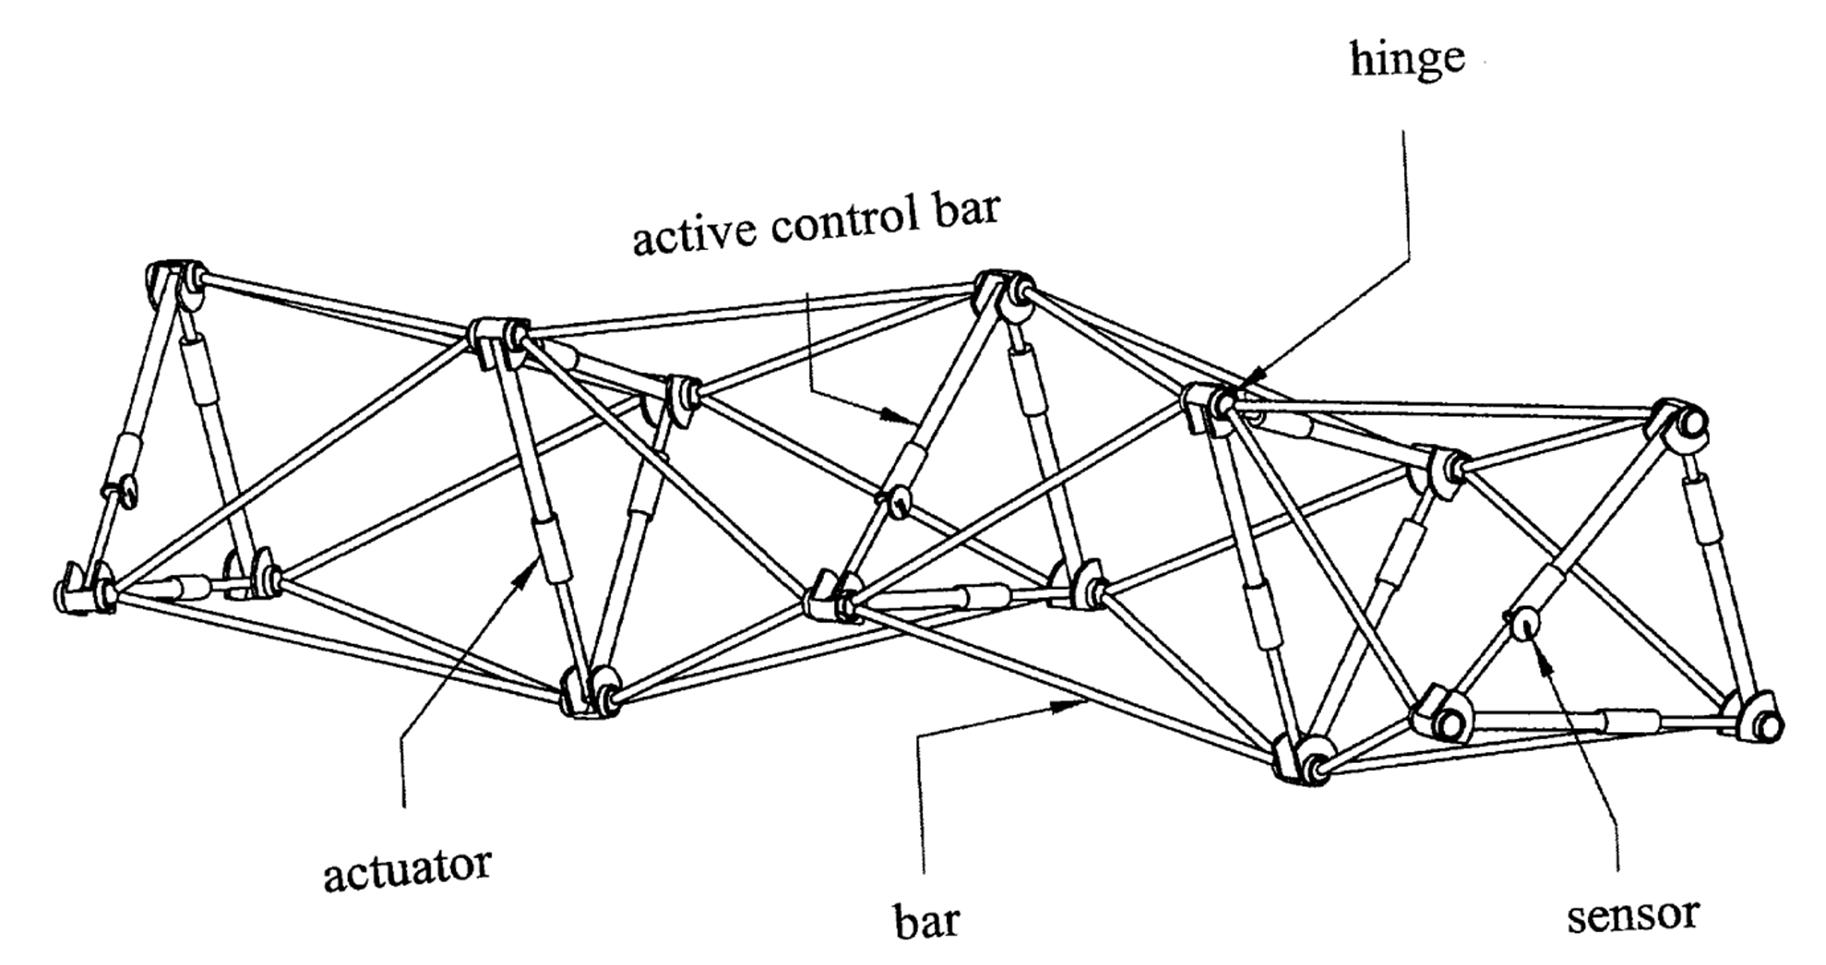
\includegraphics[height=48mm]{latex_praesentation/elements/[2]-VTT.png}
        \end{textblock*}

        Variable geometry topology (VGT) is a truss structured system that comprises actively \uline{actuated linear trusses} linked with \uline{passive rotational ball joints}.

        \medskip
        
        \begin{itemize}
            \item \textbf{Members:} Edges that are actuated linearly. \\
            has minimum and maximum lengths that are constraints.
            \item \textbf{Nodes:} Passive rotational joints. \\
            Angles between the members \\
            on joints are constrained.
        \end{itemize}

        \bigskip
        \bigskip
        \medskip
        
        \emph{Advantages:} \\
        Variable size, pass-through confined spaces.

        \medskip

        \emph{Disadvantages:} \\
        Needs a rigid actuator with high extension ratio.
 	
        \medskip

        \begin{textblock*}{5cm}(137mm,-33mm) % {block width} (coords)
        {\tiny \cite{10.1016/S0168-874X(99)00041-4}}
        \end{textblock*}
 
\end{frame}

\begin{frame}[fragile]{Realized Robots}

        \begin{textblock*}{5cm}(56mm,-30mm) % {block width} (coords)
        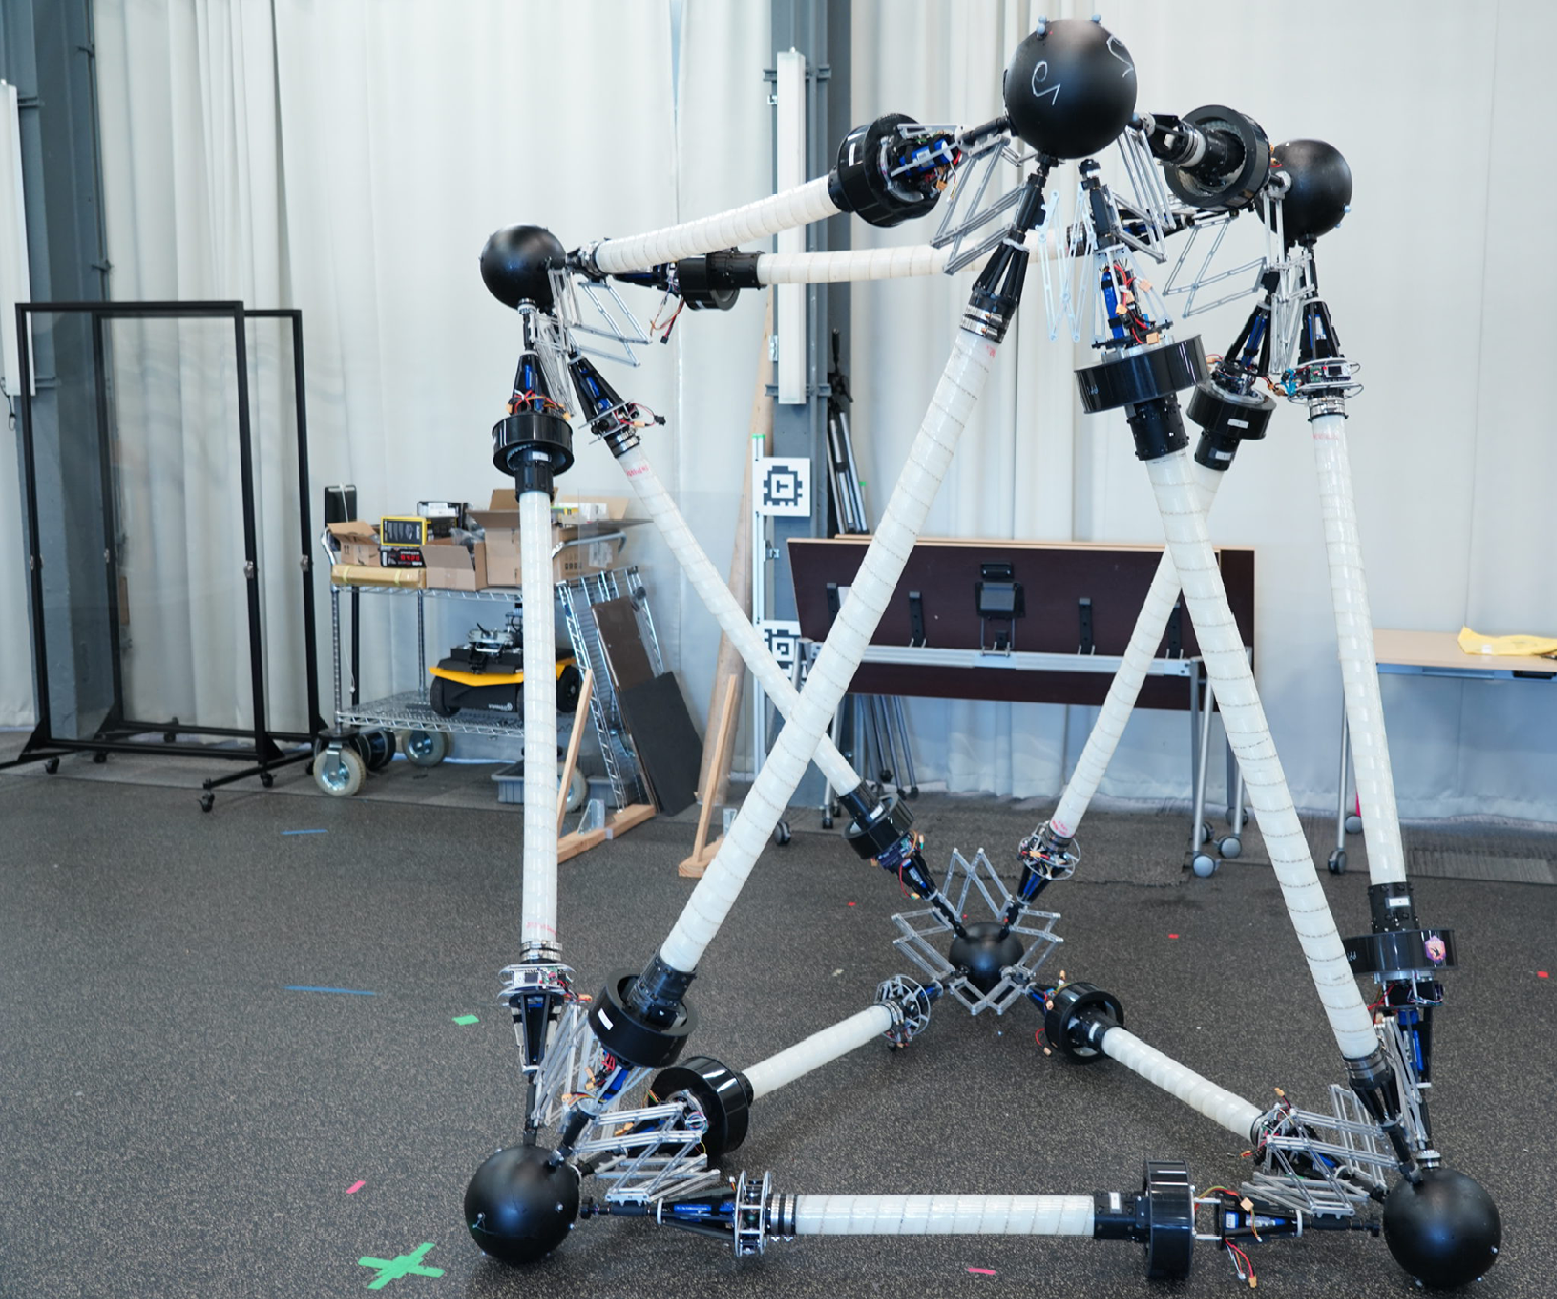
\includegraphics[height=70mm]{latex_praesentation/elements/[4]-R2.png}
        \end{textblock*}
    
        \begin{textblock*}{8cm}(0mm,-24mm) % {block width} (coords)
        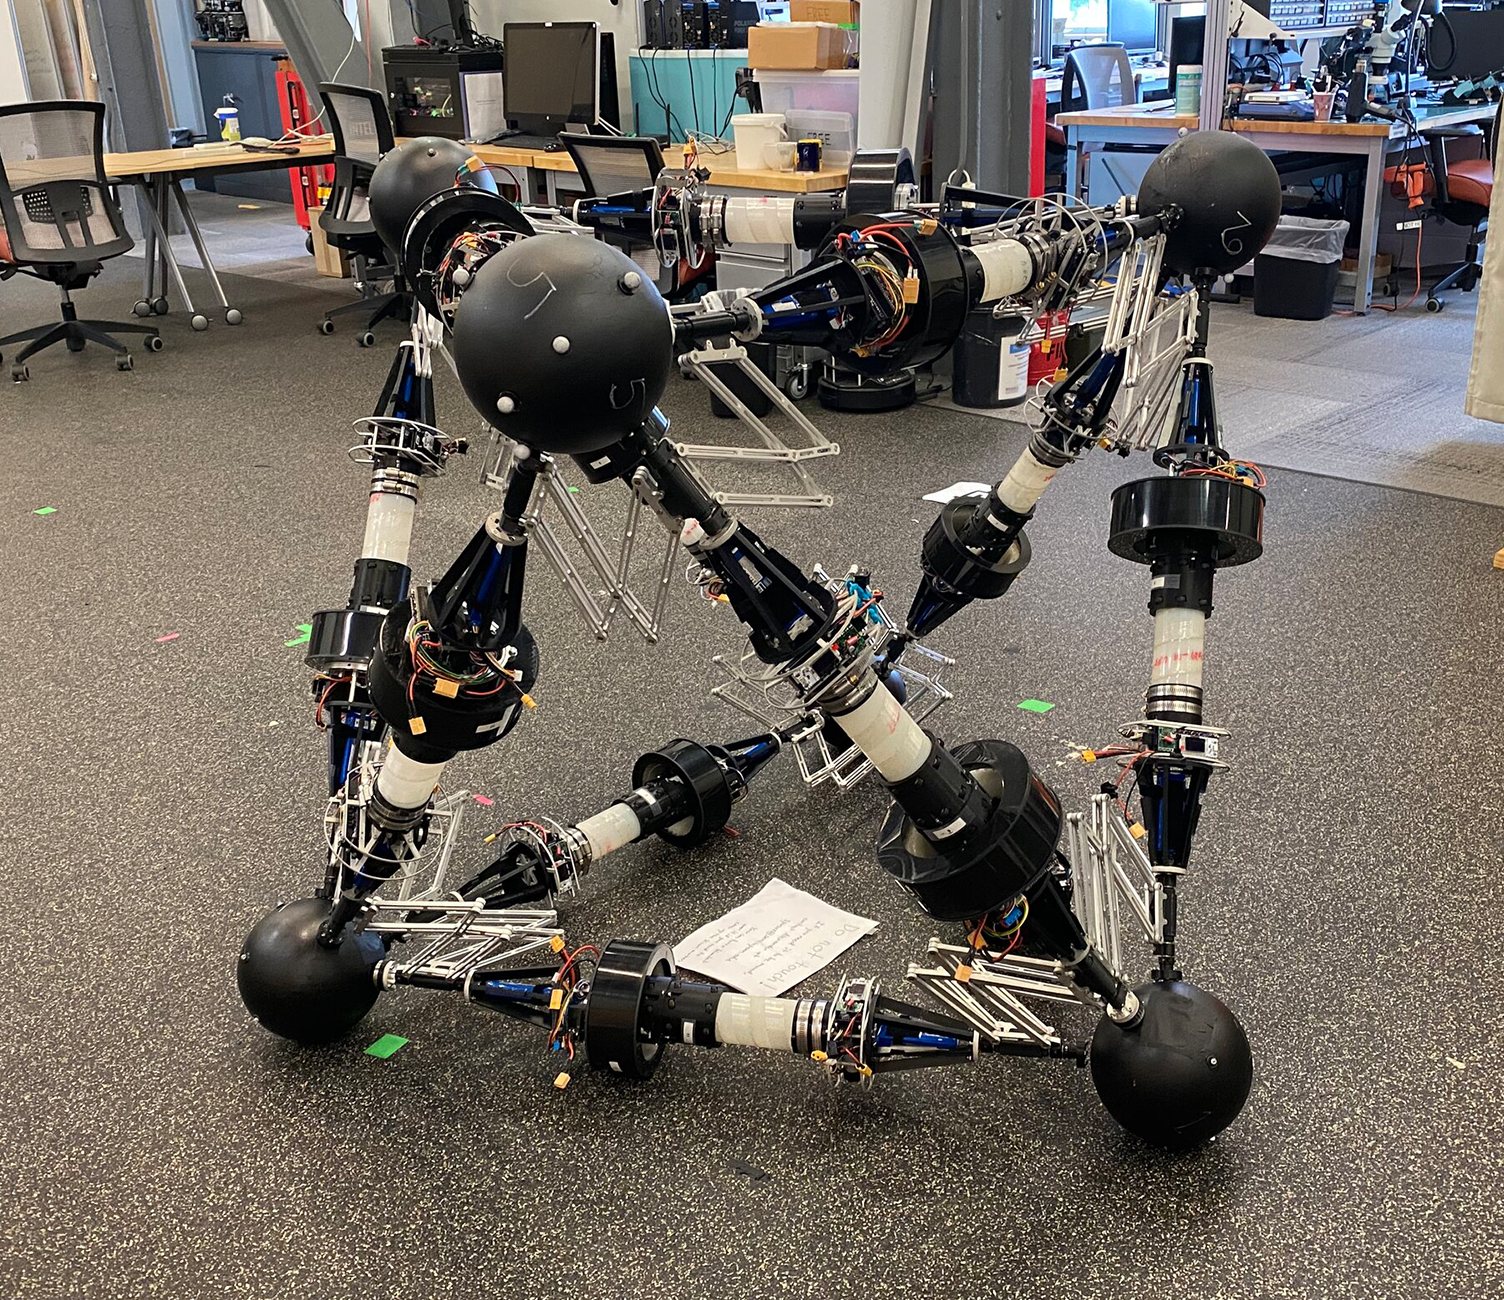
\includegraphics[height=64mm]{latex_praesentation/elements/[3]-R1.png}
        \end{textblock*}

        \begin{textblock*}{5cm}(1mm,37mm) % {block width} (coords)
        {\color{white} \tiny \cite{Guan}}
        \end{textblock*}

        \begin{textblock*}{5cm}(136.5mm,37mm) % {block width} (coords)
        {\color{white} \tiny \cite{extended}}
        \end{textblock*}
 
\end{frame}

\begin{frame}[fragile]{Realized Robots}

        \begin{textblock*}{8cm}(75mm,14mm) % {block width} (coords)
        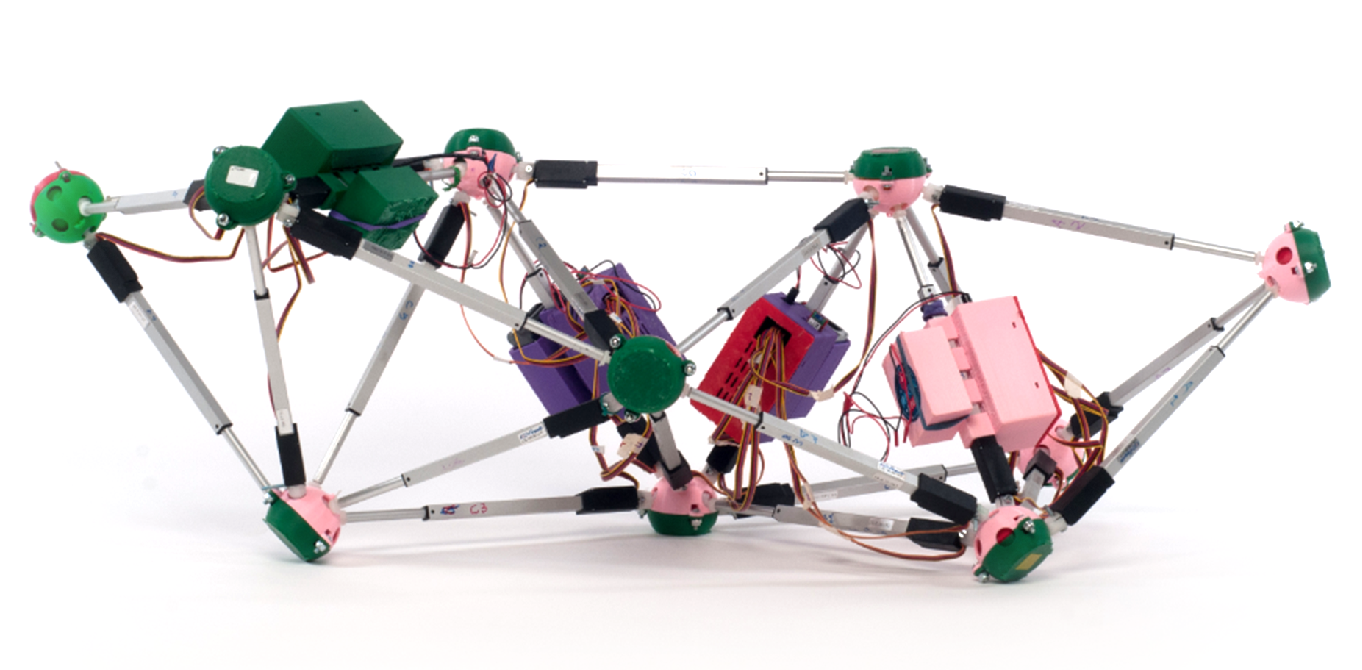
\includegraphics[height=31mm]{latex_praesentation/elements/[7]-R5.png}
        \end{textblock*} 
        
        \begin{textblock*}{8cm}(60mm,-30mm) % {block width} (coords)
        {\color{white}\href{https://youtu.be/x40DKmI6l84}{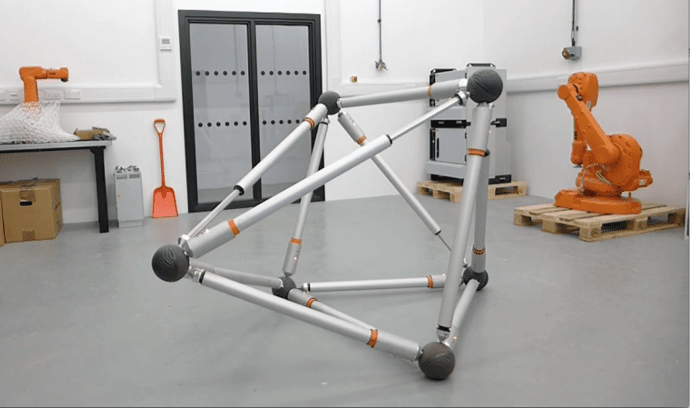
\includegraphics[height=46mm]{elements/[6]-R4.png}}}
        \end{textblock*}
    
        \begin{textblock*}{5cm}(0mm,-24mm) % {block width} (coords)
        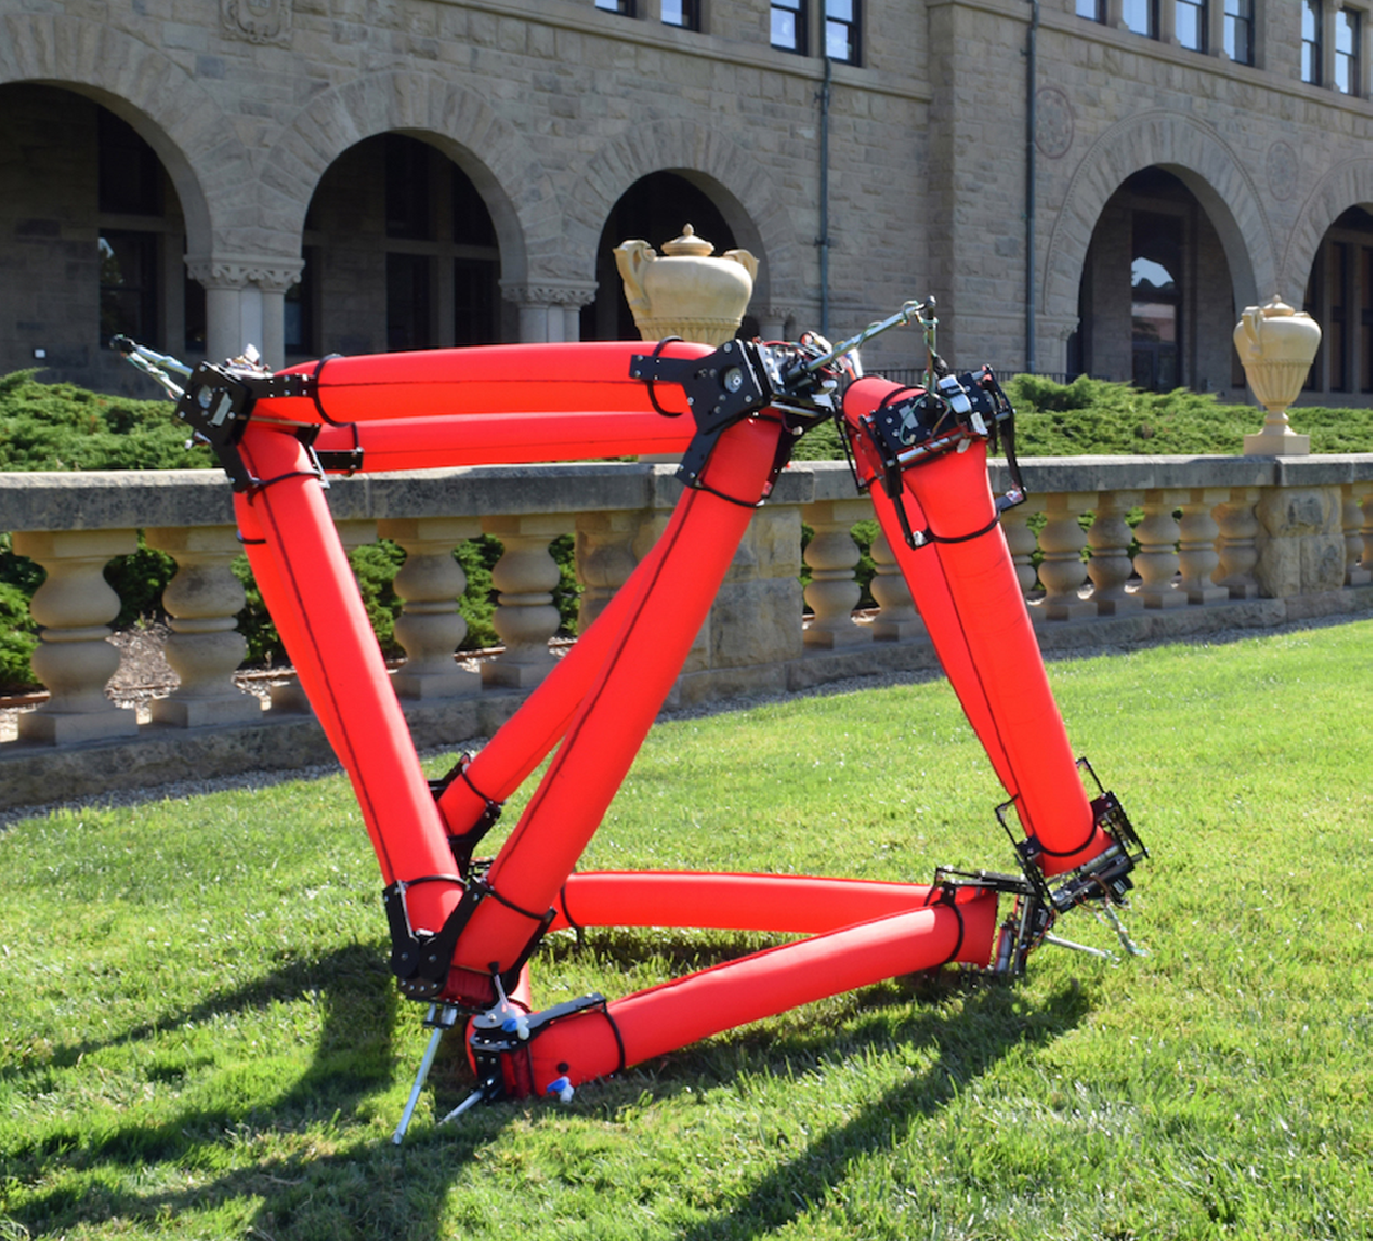
\includegraphics[height=64mm]{latex_praesentation/elements/[5]-R3.png}
        \end{textblock*}

        \begin{textblock*}{5cm}(1mm,37mm) % {block width} (coords)
        {\color{white} \tiny \cite{SHAPE}}
        \end{textblock*}

        \begin{textblock*}{5cm}(134.5mm,13mm) % {block width} (coords)
        {\color{white} \tiny \cite{william-bondin}}
        \end{textblock*}

        \begin{textblock*}{5cm}(134.5mm,38mm) % {block width} (coords)
        {\color{black} \tiny \cite{10.1145/3448326.3448332}}
        \end{textblock*}
 
\end{frame}


\section{Research Question}

\begin{frame}[fragile]{\textbf{Locomotion Strategy for the VGT Robot} \hfill \fontsize{8}{8}\selectfont RESEARCH QUESTION}
    
        \begin{textblock*}{5cm}(71mm,16mm) % {block width} (coords)
        % 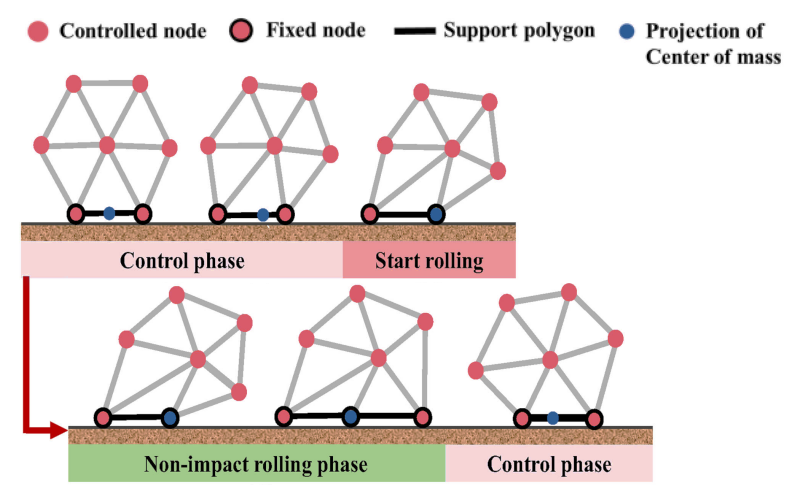
\includegraphics[height=44mm]{elements/[9]-LOCO.png}}
        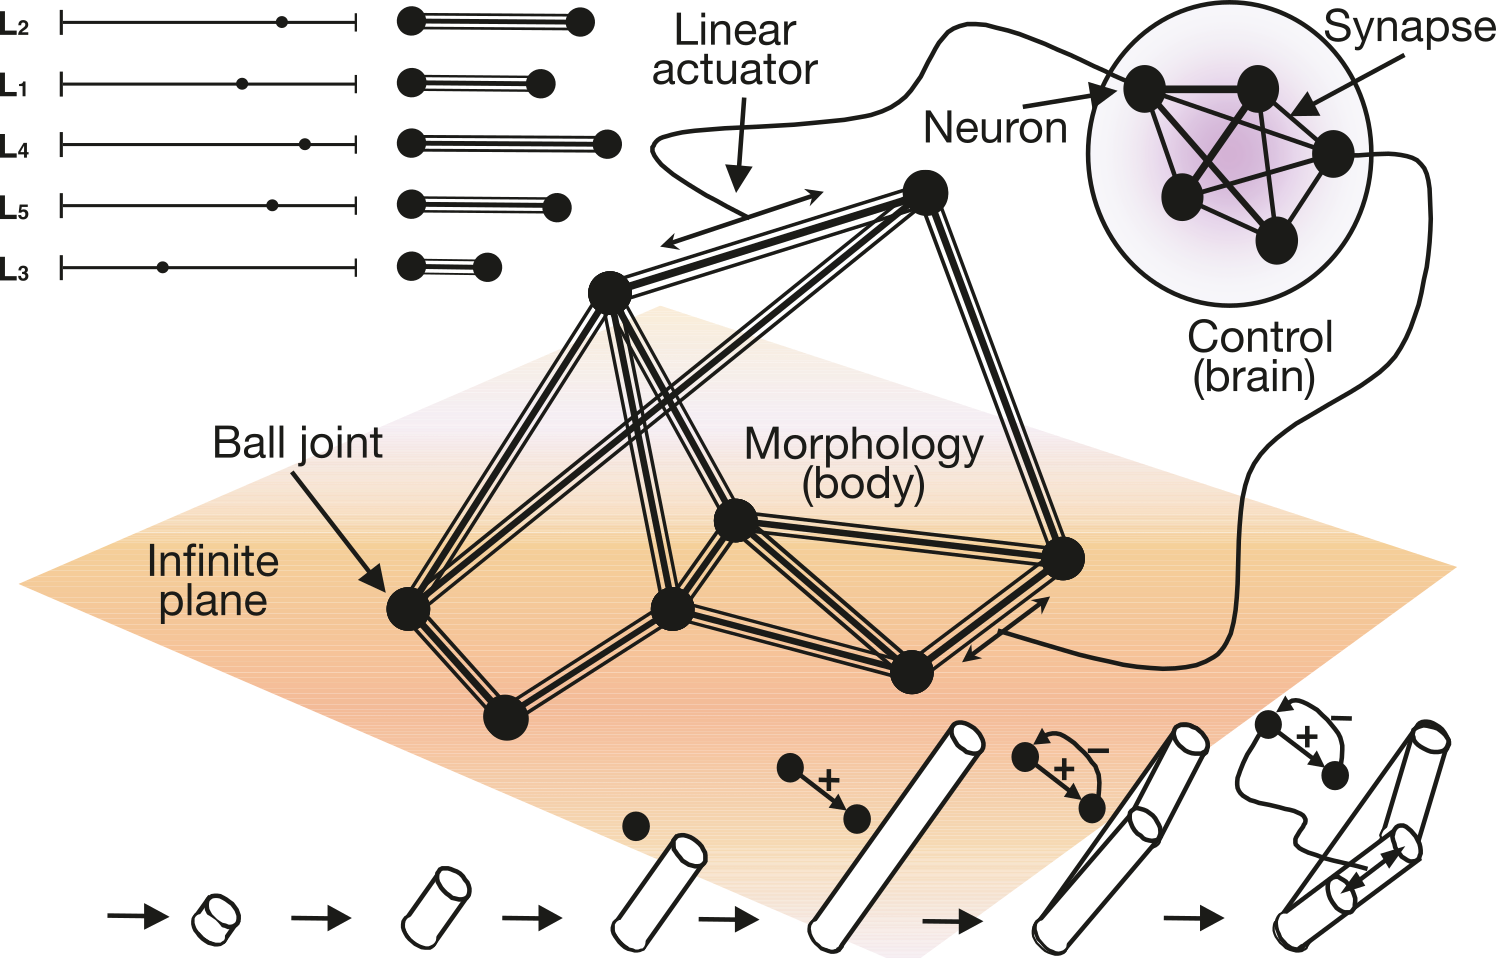
\includegraphics[height=42mm]{elements/[2].png}
        \end{textblock*}

         \uline{\textit{Development of a reinforcement learning based locomotion strategy for truss robots.}}
         This involves coordinating the movement of various parts in a specific sequence, similar to how serpents or mammals move, where intricate coordination is necessary.

        \bigskip
        
        \begin{tikzpicture}
          % \draw [->] (1,1) |-  (2,-3) node[pos=0.25,above,sloped] {Idea Development};
            \draw [->] (1,0) node[yshift=1.5cm,rotate=90] {Idea Development} |-  (1.5,-1.1);
        \end{tikzpicture}

        \begin{textblock*}{60mm}(7mm,-40mm)
        The structure consists of $\mathrm{N}$ linear actuators, each with a single degree of freedom ($\mathrm{DoF}$), interconnected with passive joints.
        
        \begin{enumerate}
            \item \textit{Model-Based/Free RL:} Single topology, baseline for comparison.
            \item \textit{Modular Control Policy RL:} Multiple topology, generalizability.
            \item \textit{Multi-Agent Policy RL:} Each member is an individual agent.
        \end{enumerate}
        
        \end{textblock*}
        
        \begin{textblock*}{5cm}(135mm, -1mm) % {block width} (coords)
        {\tiny \cite{Lipson2000}}
        \end{textblock*}
        \vfill
 
\end{frame}

\section{Literature Review}

\begin{frame}[fragile]{\fontsize{10}{10}\selectfont\textbf{[Non-impact Rolling Locomotion of a Variable Geometry Truss]} \hfill \fontsize{8}{8}\selectfont LITERATURE REVIEW \newline [2019]}
    
        \begin{textblock*}{5cm}(0mm,12mm) % {block width} (coords)
        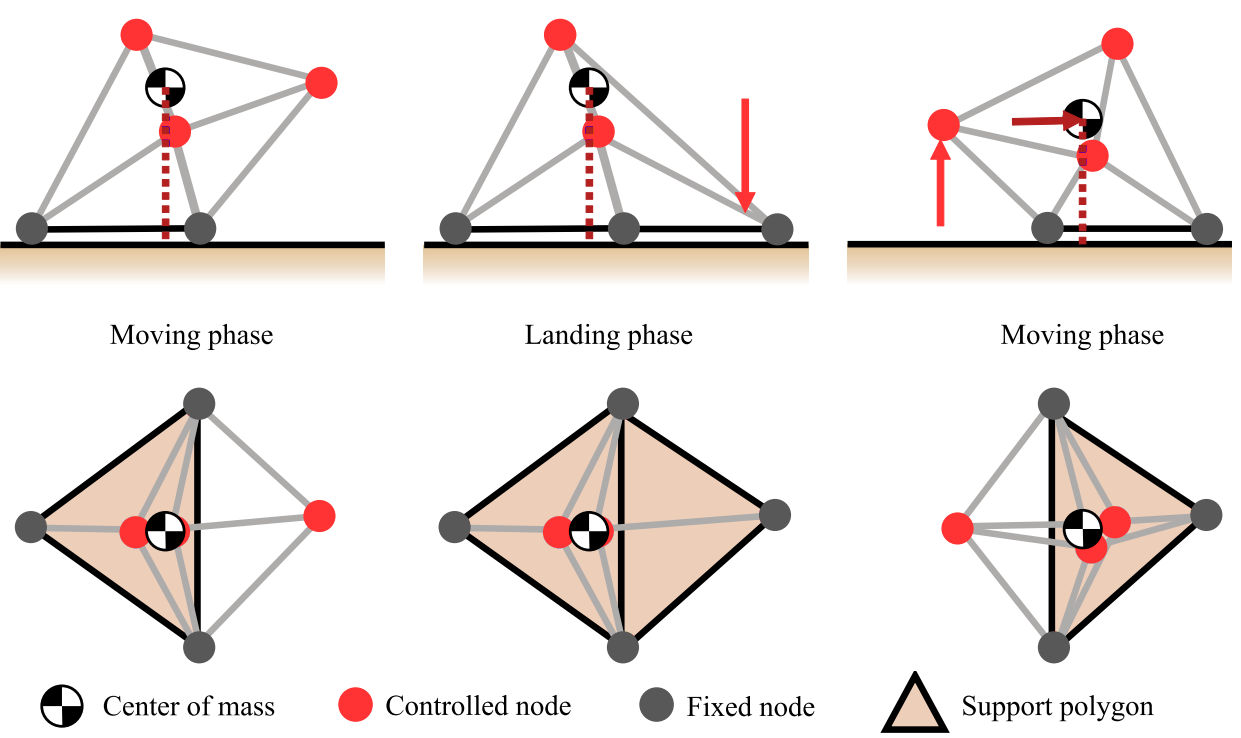
\includegraphics[height=46mm]{elements/[8]-LOCO.png}
        \end{textblock*}

        \begin{textblock*}{5cm}(90mm,-3mm) % {block width} (coords)
        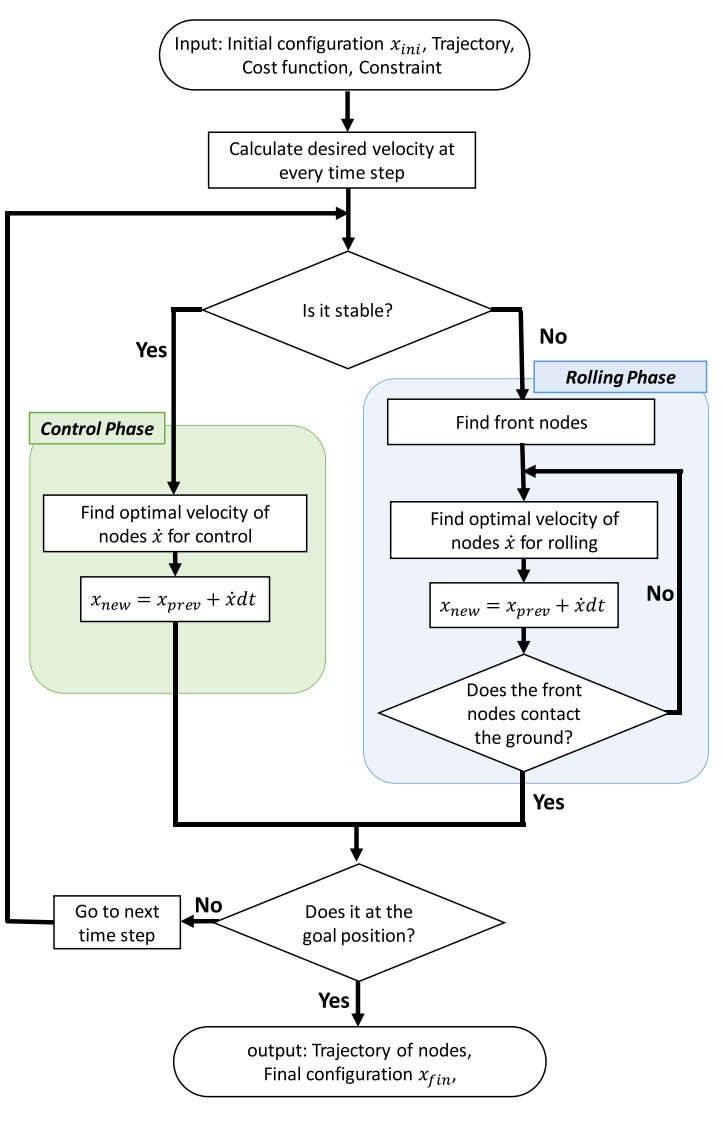
\includegraphics[height=65mm]{elements/[10]-LOCO.png}
        \end{textblock*}

        \begin{textblock*}{87mm}(0mm,-2mm)
        The velocity of nodes is optimized to move the center of mass given the desired velocity. The member velocities are calculated and actuated accordingly.$^{\text{\cite{Usevitch}}}$
        \end{textblock*}

        \begin{textblock*}{5cm}(133mm, 58mm) % {block width} (coords)
        {\tiny \cite{8610002}}
        \end{textblock*}

        \begin{textblock*}{5cm}(75mm, 58mm) % {block width} (coords)
        {\tiny \cite{bb}}
        \end{textblock*}
        
        \vspace{52mm}
\end{frame}

\begin{frame}[fragile]{\fontsize{10}{10}\selectfont\textbf{[Learning Modular Robot Control Policies]} \hfill \fontsize{8}{8}\selectfont LITERATURE REVIEW \newline [2023]}
    
        \begin{textblock*}{5cm}(0mm,17mm) % {block width} (coords)
        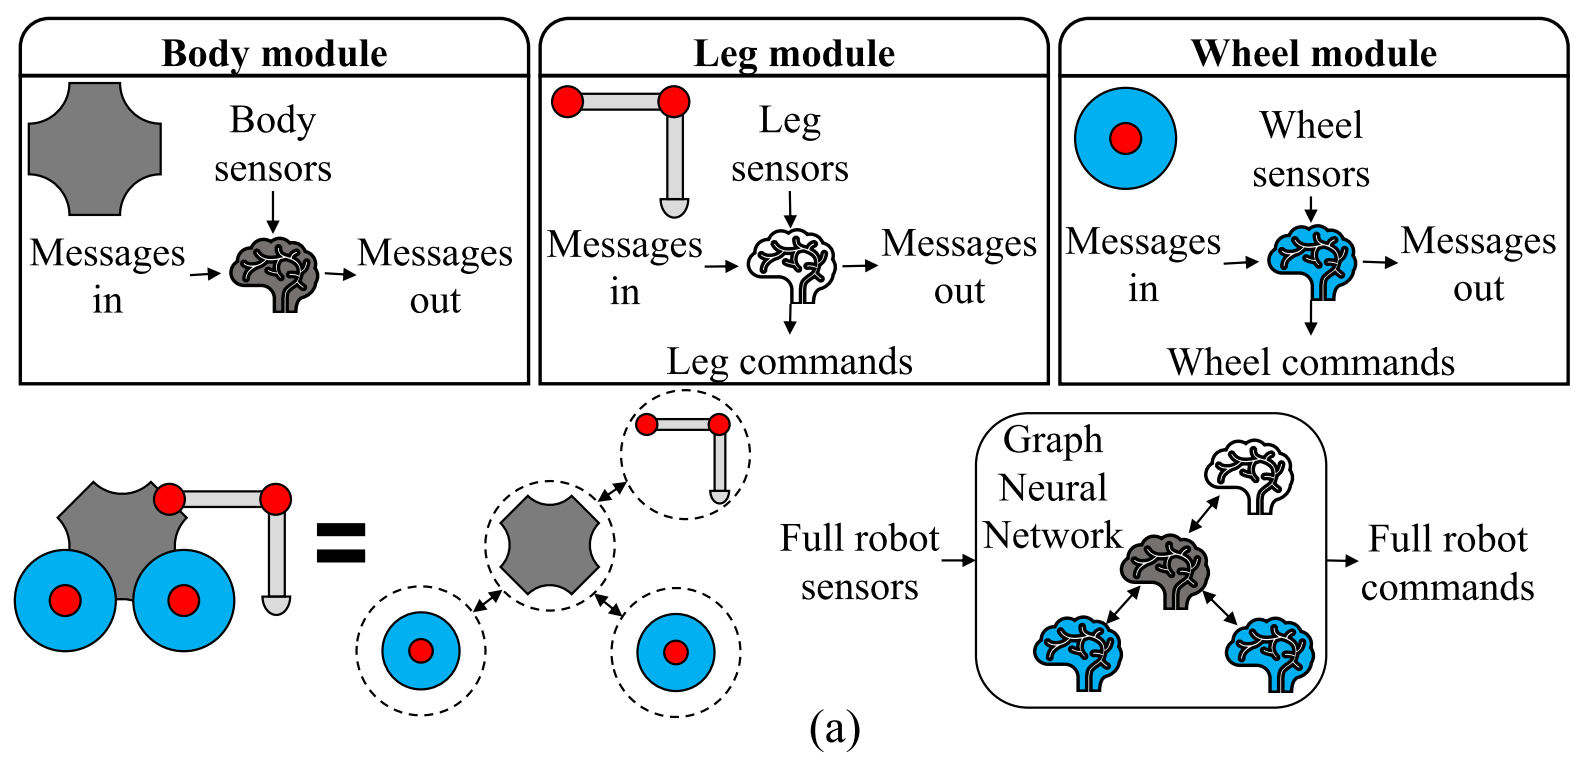
\includegraphics[height=40mm]{elements/choset-II.png}
        \end{textblock*}

        \begin{textblock*}{5cm}(85mm,-3mm) % {block width} (coords)
        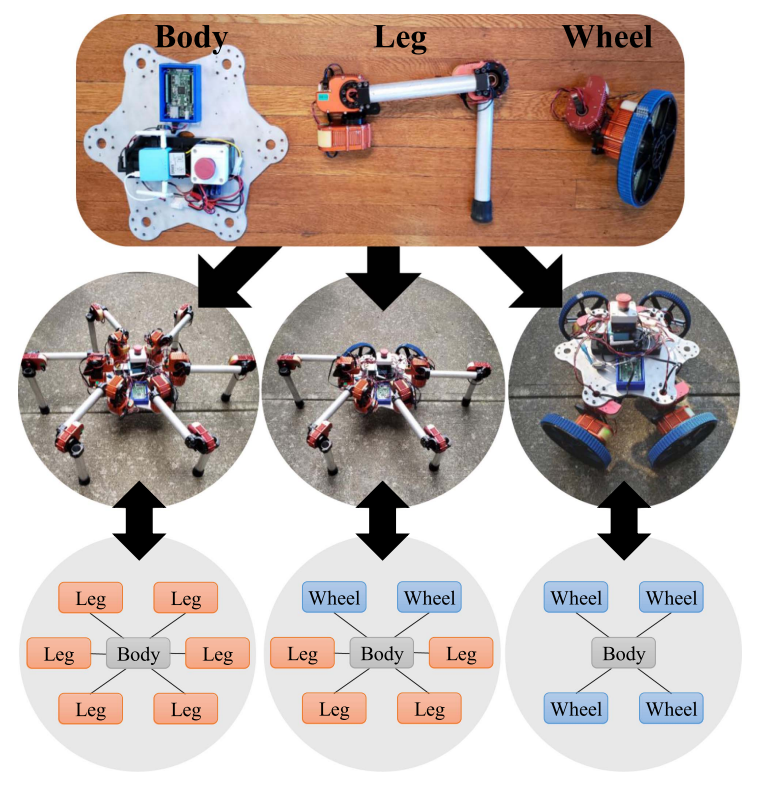
\includegraphics[height=59mm]{elements/choset.png}
        \end{textblock*}

        \begin{textblock*}{87mm}(0mm,-2mm)
        Modular robots need specific control policies for each design, which becomes impractical for scalability. A modular policy framework allows for a single training process to adapt to various hardware arrangements and control different designs efficiently.$^{\text{\cite{10167528}}}$
        \end{textblock*}

        \begin{textblock*}{5cm}(133mm, 58mm) % {block width} (coords)
        {\tiny \cite{10167528}}
        \end{textblock*}

        \begin{textblock*}{5cm}(75mm, 58mm) % {block width} (coords)
        {\tiny \cite{10167528}}
        \end{textblock*}
        
        \vspace{52mm}
\end{frame}

\begin{frame}[fragile]{\fontsize{10}{10}\selectfont\textbf{[Distributed Coach-Based RL Controller for Snake Robot Locomotion]} \hfill \fontsize{8}{8}\selectfont LITERATURE \newline [2022]}


        \begin{textblock*}{5cm}(78mm,-11mm) % {block width} (coords)
        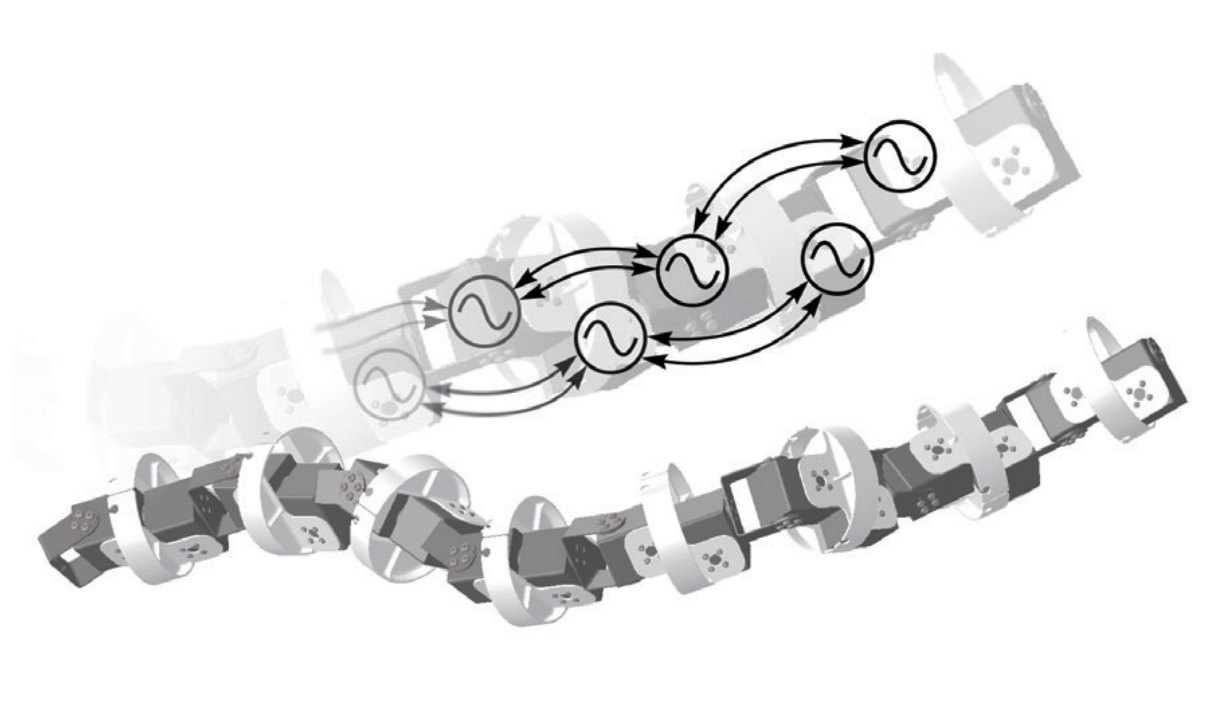
\includegraphics[height=38mm,angle=50,origin=c]{elements/snake-3.png}
        \end{textblock*}
        
        \begin{textblock*}{5cm}(0mm,17mm) % {block width} (coords)
        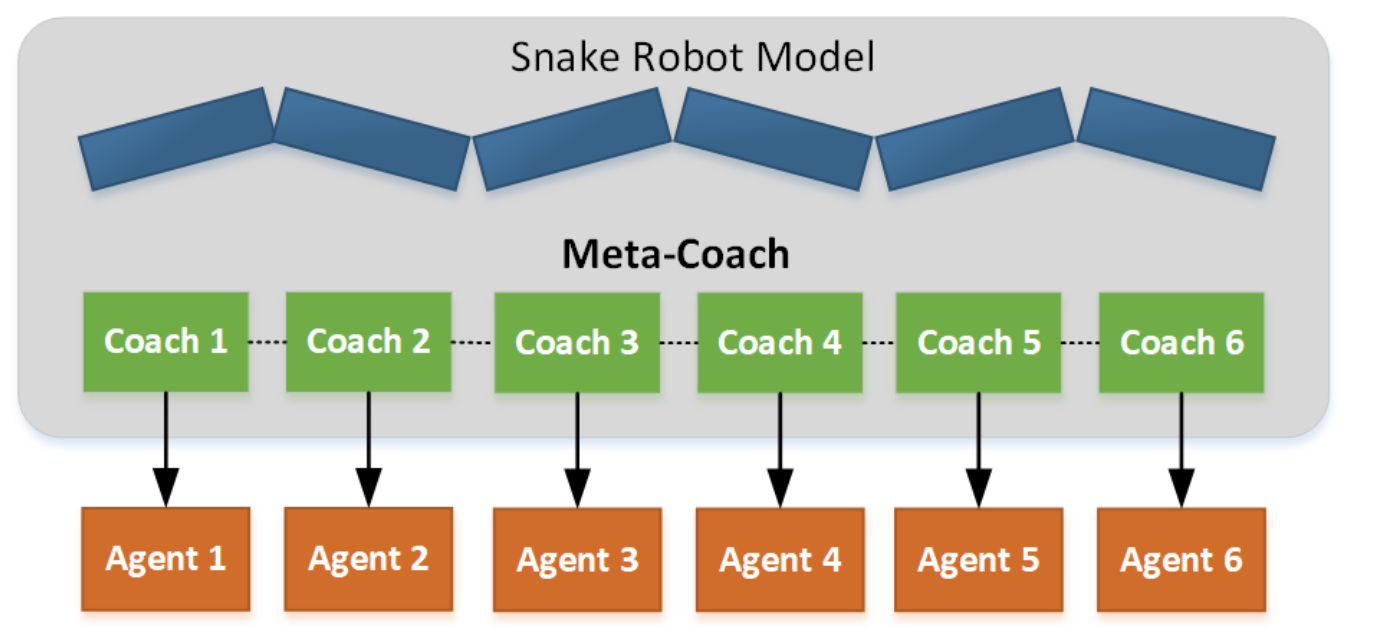
\includegraphics[height=40mm]{elements/snake-1.png}
        \end{textblock*}

        \begin{textblock*}{87mm}(0mm,-2mm)
        Snake robot control with RL is underexplored due to high freedom redundancy. Existing methods use asynchronous joint state representations. A new solution introduces a distributed coach-based learning approach to address these challenges.$^{\text{\cite{9981749}}}$
        \end{textblock*}

        \begin{textblock*}{5cm}(133mm, 58mm) % {block width} (coords)
        {\tiny \cite{9517436}}
        \end{textblock*}

        \begin{textblock*}{5cm}(75mm, 58mm) % {block width} (coords)
        {\tiny \cite{9981749}}
        \end{textblock*}
        
        \vspace{52mm}
\end{frame}

\section{Methodology \& Algorithms}

\begin{frame}[fragile]{\textbf{Developmental Procedure} \hfill \fontsize{8}{8}\selectfont Methods / Algorithms}
    
        \begin{textblock*}{5cm}(0mm,9mm) % {block width} (coords)
        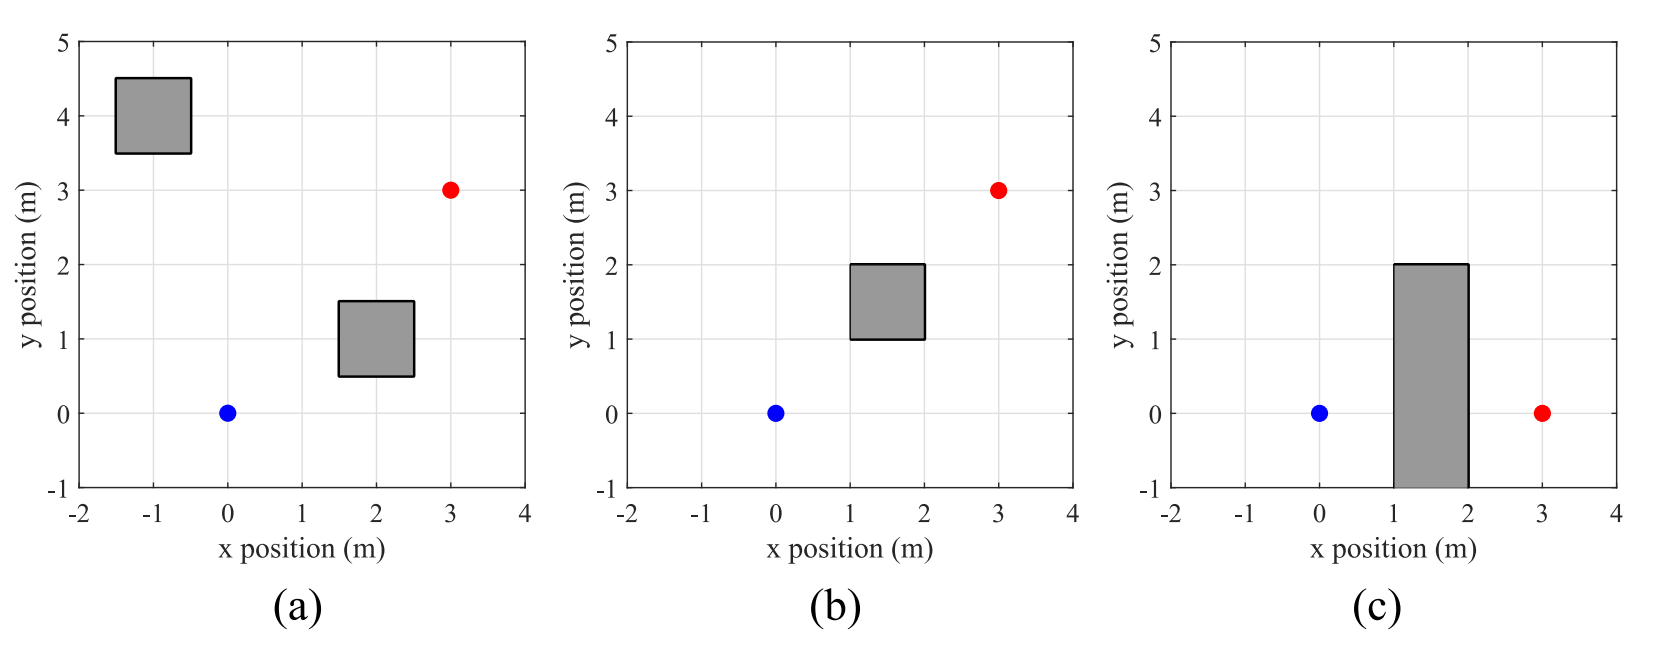
\includegraphics[height=33mm]{elements/[12]-PLAN.png}
        \end{textblock*}

        \begin{textblock*}{5cm}(92mm,-30mm) % {block width} (coords)
        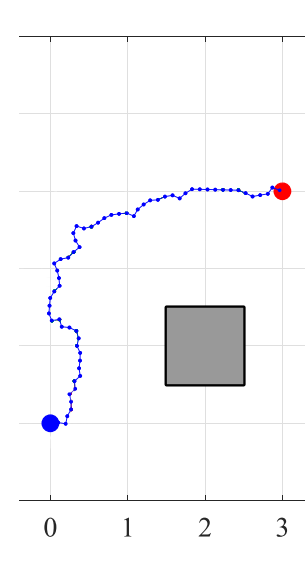
\includegraphics[height=74mm]{elements/[13]-PLAN.png}
        \end{textblock*}

        \begin{textblock*}{87mm}(0mm,-20mm)
         Having defined the truss structure and the locomotion algorithm, the path planning comes next. Start by describing the workspace.  
        
        \begin{itemize}
            \item 2D Plane
            \item Polygonal Obstacles
            \item Initial point and a goal point
        \end{itemize}

        \end{textblock*}

        \begin{textblock*}{25mm}(46mm,-8mm)
        \begin{equation*}
            \begin{rcases}
              \text{\color{white}-}\\
              \text{\color{white}-}\\
            \end{rcases}   
            \begin{array}{l}
              \text{Find a path for}\\
              \text{center of mass to follow}\\
            \end{array}
        \end{equation*}
        \end{textblock*}

        \begin{textblock*}{5cm}(133mm, 36mm) % {block width} (coords)
        {\tiny \cite{bb}}
        \end{textblock*}

        \begin{textblock*}{5cm}(86mm, 36mm) % {block width} (coords)
        {\tiny \cite{bb}}
        \end{textblock*}

\end{frame}


\begin{frame}[fragile]{\textbf{Polygonal-RRT Path Planning (PRT)}}
    
        \begin{textblock*}{5cm}(9mm,9mm) % {block width} (coords)
        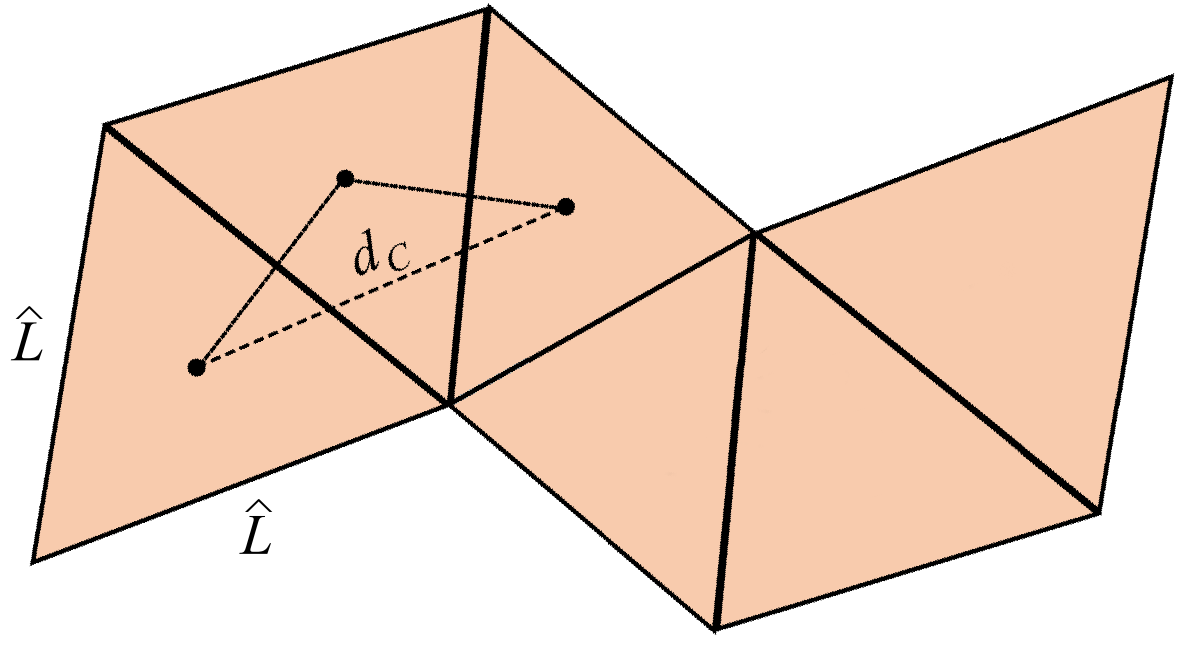
\includegraphics[height=26mm]{elements/[15]-PRT.png}
        \end{textblock*}

        \begin{textblock*}{5cm}(64mm,-13mm) % {block width} (coords)
        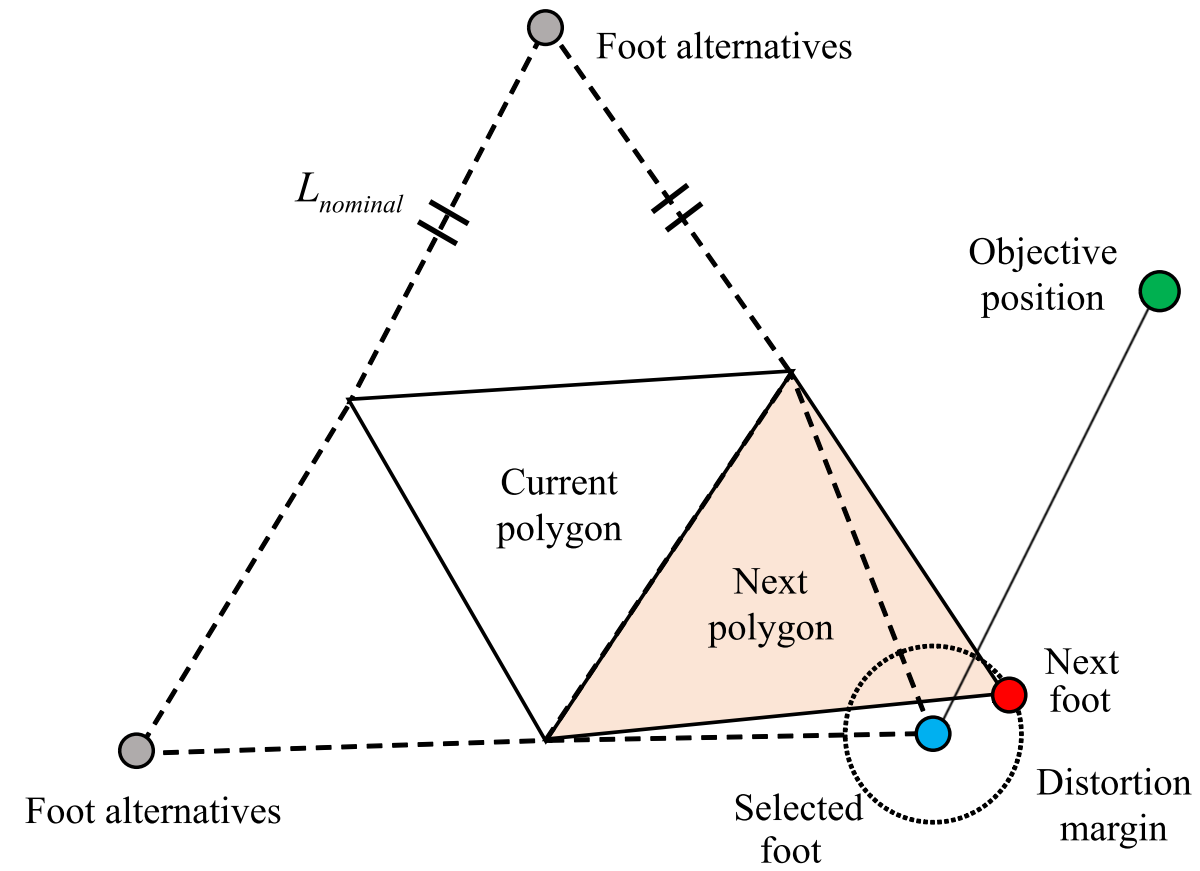
\includegraphics[height=55mm]{elements/[14]-PRT.png}
        \end{textblock*}

        \begin{textblock*}{130mm}(0mm,-20mm)
        One can incorporate the geometry of the topology into the random tree search algorithm. 
        \vspace{4.5mm}
        \begin{itemize}
            \item Generate a tree that consist of polygons.
            \item Select the next branch from 3 possible foot nodes.
            \item Terminate when the goal is within the support polygon.
        \end{itemize}
        \end{textblock*}


        \begin{textblock*}{5cm}(128mm, -10mm) % {block width} (coords)
        {\tiny \cite{bb}}
        \end{textblock*}

\end{frame}


\begin{frame}[fragile]{\textbf{Polygonal-RRT Path Planning (PRT)}}
    
        \begin{textblock*}{5cm}(0mm,-15mm) % {block width} (coords)
        \href{https://youtu.be/LATWgYy7ye0?si=a48bX9n5iTIcAjNj&t=29}{
        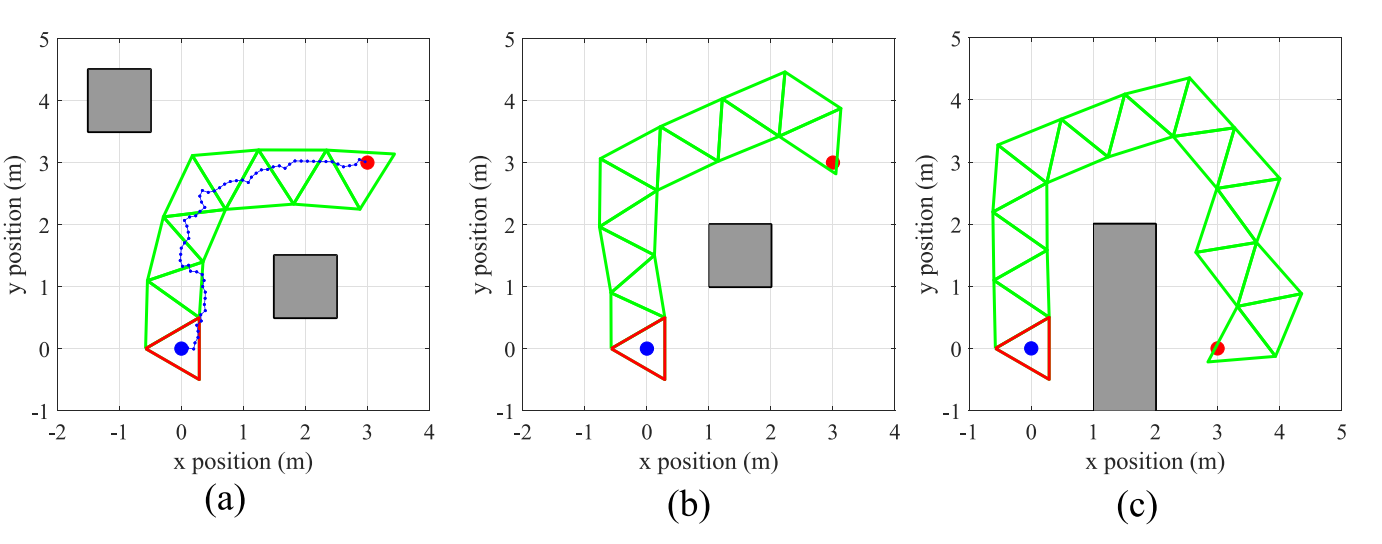
\includegraphics[height=33mm]{elements/[17]-PRT.png}}
        \end{textblock*}

        \begin{textblock*}{5cm}(85mm,-32mm) % {block width} (coords)
        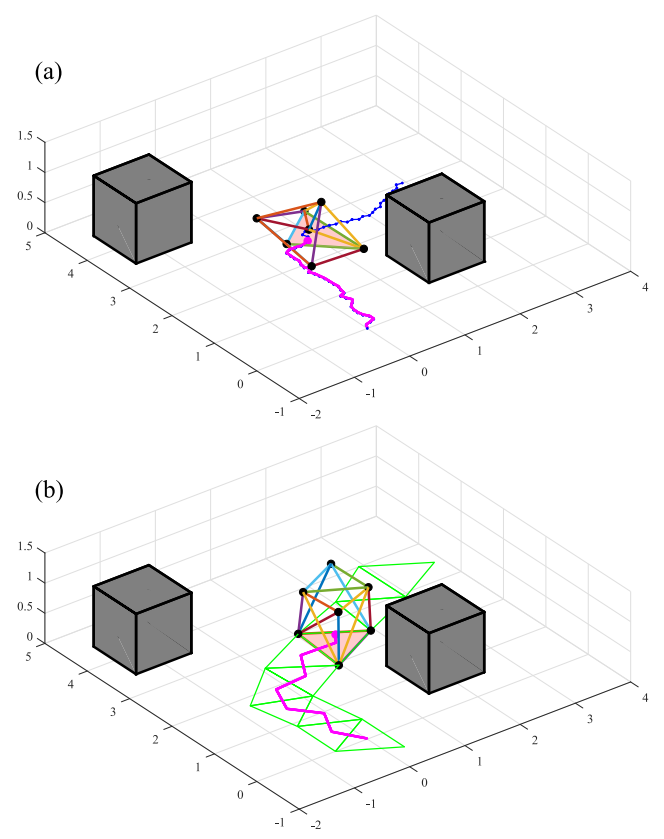
\includegraphics[height=70mm]{elements/[16]-PRT.png}
        \end{textblock*}

        \begin{textblock*}{5cm}(0mm,15mm) % {block width} (coords)
        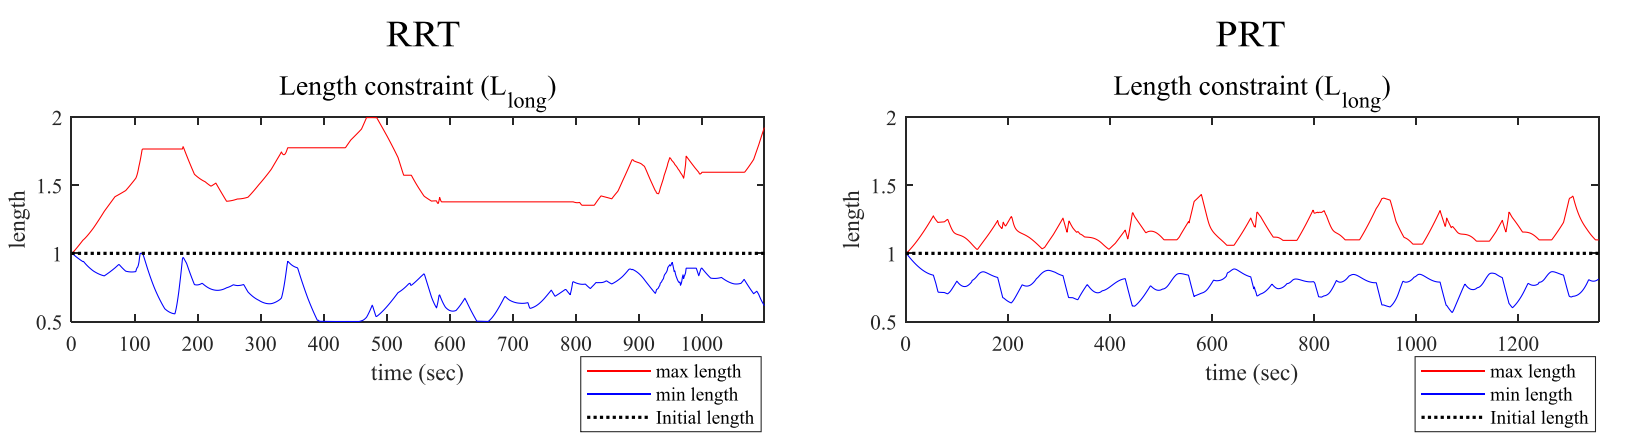
\includegraphics[height=22.2mm]{elements/[18]-PRT.png}
        \end{textblock*}
        
        \begin{textblock*}{130mm}(0mm,-22mm)
        Comparative results differentiating the PRT and the RRT. 
        % \vspace{4.5mm}
        % \begin{itemize}
        %     \item Generate a tree that consist of polygons.
        %     \item Select the next branch from 3 possible foot nodes.
        %     \item Terminate when the goal is within the support polygon.
        % \end{itemize}
        \end{textblock*}

        \begin{textblock*}{5cm}(3mm, 13mm) % {block width} (coords)
        {\tiny \cite{bb}}
        \end{textblock*}
        
        \begin{textblock*}{5cm}(3mm, 34mm) % {block width} (coords)
        {\tiny \cite{bb}}
        \end{textblock*}
        
        \begin{textblock*}{5cm}(136mm, 34mm) % {block width} (coords)
        {\tiny \cite{bb}}
        \end{textblock*}

\end{frame}


\begin{frame}[fragile]{\textbf{Discussions on PRT Results}}

        \begin{textblock*}{130mm}(0mm,-22mm)
        Problems and ideas to be thought on. 
        \medskip
        \begin{itemize}
            \item The selected tree branch size is too small for the RRT.
            \item Rotating around the CM mechanism can be added.
            \item A direction concept could be beneficial.
            \item CM trajectory can be smoothed.
            \item Why choose adjacent adjacent polygons as the support ?
            % \item Locomotion uses adjacent polygons as support polygon. 
        \end{itemize}
        \end{textblock*}

        \begin{textblock*}{5cm}(95mm,-30mm) % {block width} (coords)
        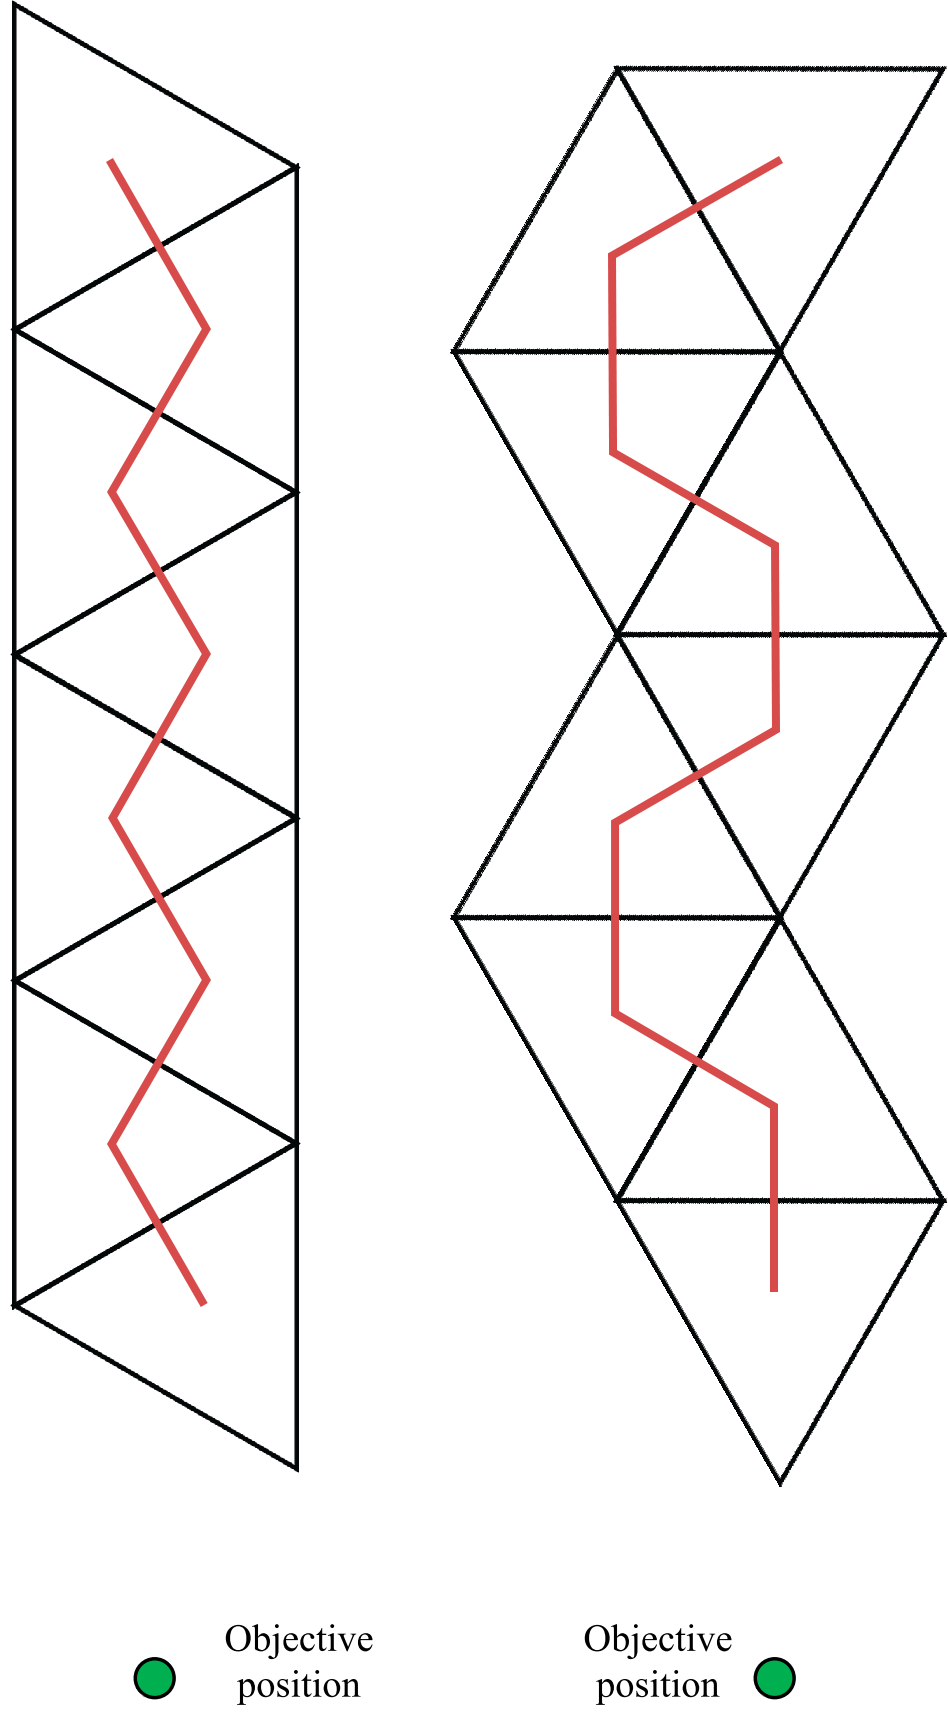
\includegraphics[height=70mm]{elements/[19]-PRT.png}
        \end{textblock*}

        \begin{textblock*}{5cm}(13mm,10mm) % {block width} (coords)
        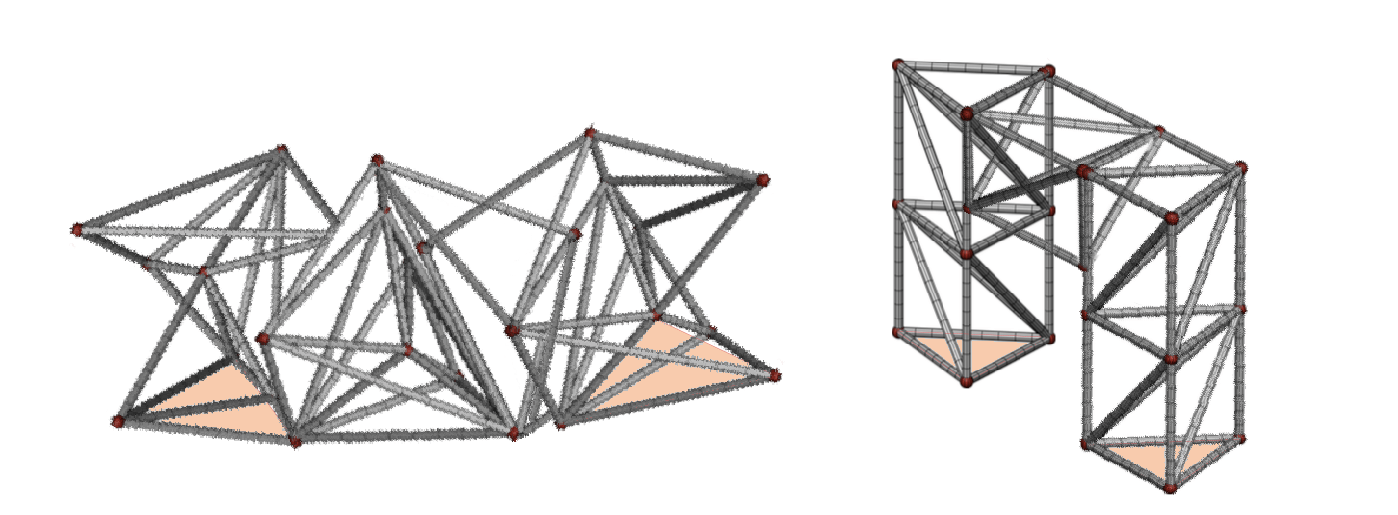
\includegraphics[height=28mm]{elements/[19-2]-PRT.png}
        \end{textblock*}

\end{frame}


\section{Risks \& Limitations}

\begin{frame}[fragile]{\textbf{Assessing the Feasibility} \hfill \fontsize{8}{8}\selectfont RISKS / LIMITATIONS}
    
        \begin{textblock*}{5cm}(9mm,12.7mm) % {block width} (coords)
        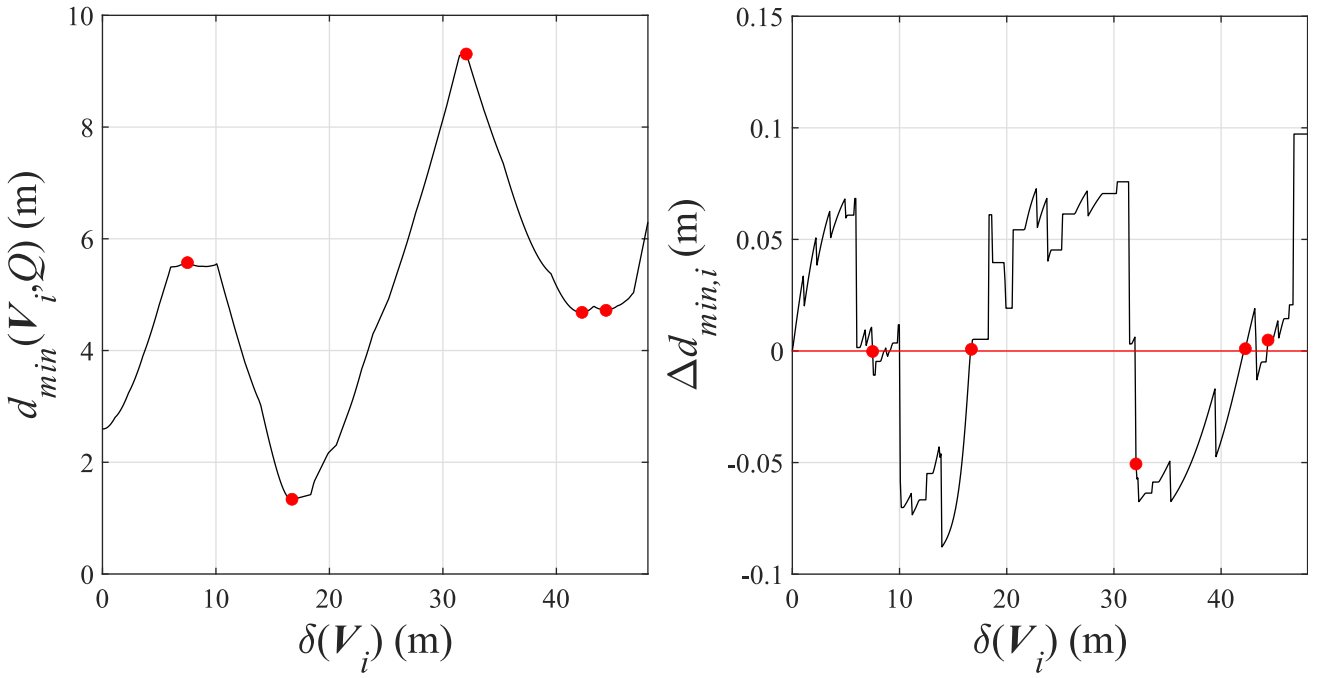
\includegraphics[height=30mm]{elements/[21]-PRT-V.png}
        \end{textblock*}

        \begin{textblock*}{5cm}(76mm,-23mm) % {block width} (coords)
        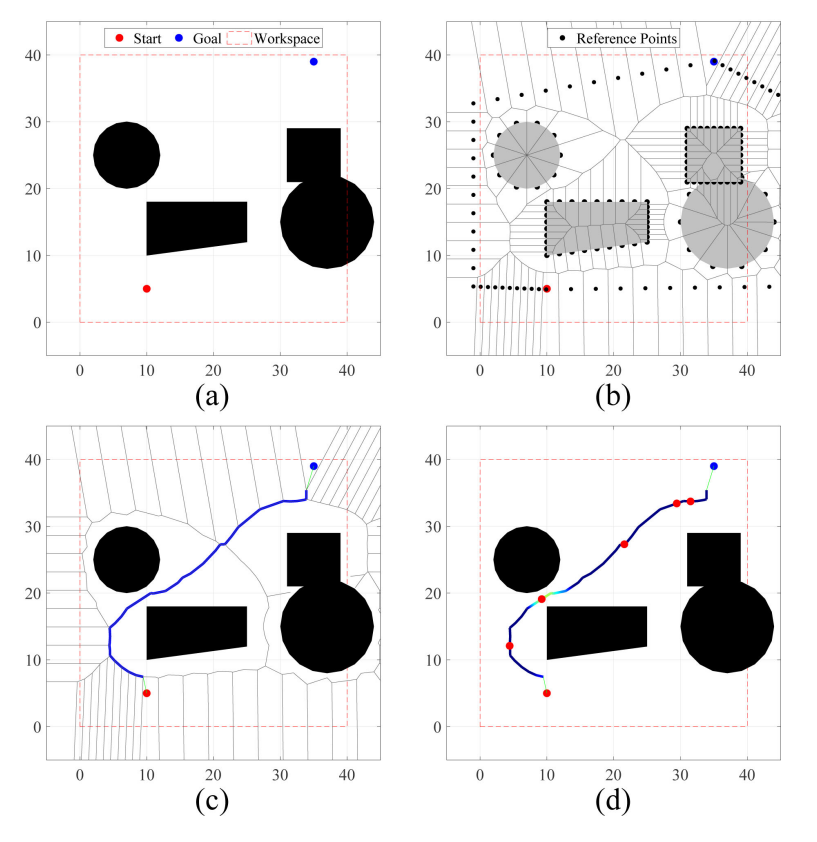
\includegraphics[height=68mm]{elements/[20]-PRT-V.png}
        \end{textblock*}

        \begin{textblock*}{74mm}(0mm,-20mm)
        One of the advantages of the physical topology is the \uline{size changing aspect}. The setting is still the same, but the question is when to change the size ?
        \vspace{2mm}
        \begin{enumerate}
            \item Voronoi and Dijkstra's algorithm to find a path.
            \item Classify the distance to the closest object.
            \item Find \alert{stepover} points that signal a size change.
        \end{enumerate}
        \end{textblock*}


        \begin{textblock*}{5cm}(135.5mm, 41mm) % {block width} (coords)
        {\tiny \cite{9477154}}
        \end{textblock*}

        \begin{textblock*}{5cm}(13mm, 41mm) % {block width} (coords)
        {\tiny \cite{9477154}}
        \end{textblock*}

        \vspace{10mm}

\end{frame}


\begin{frame}[fragile]{\textbf{Variable Polygon Size PRT Algorithm}}
    
        \begin{textblock*}{5cm}(5mm,12.7mm) % {block width} (coords)
        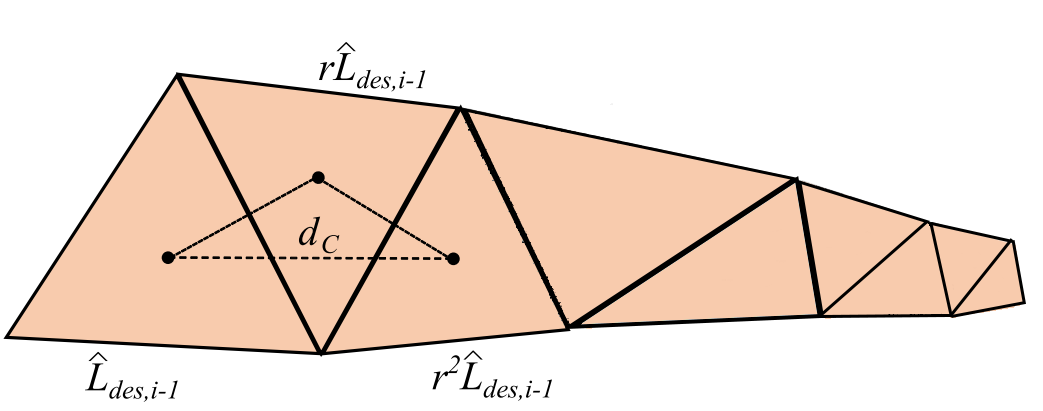
\includegraphics[height=30mm]{elements/[22]-PRT-V.png}
        \end{textblock*}

        \begin{textblock*}{5cm}(90mm,-28mm) % {block width} (coords)
        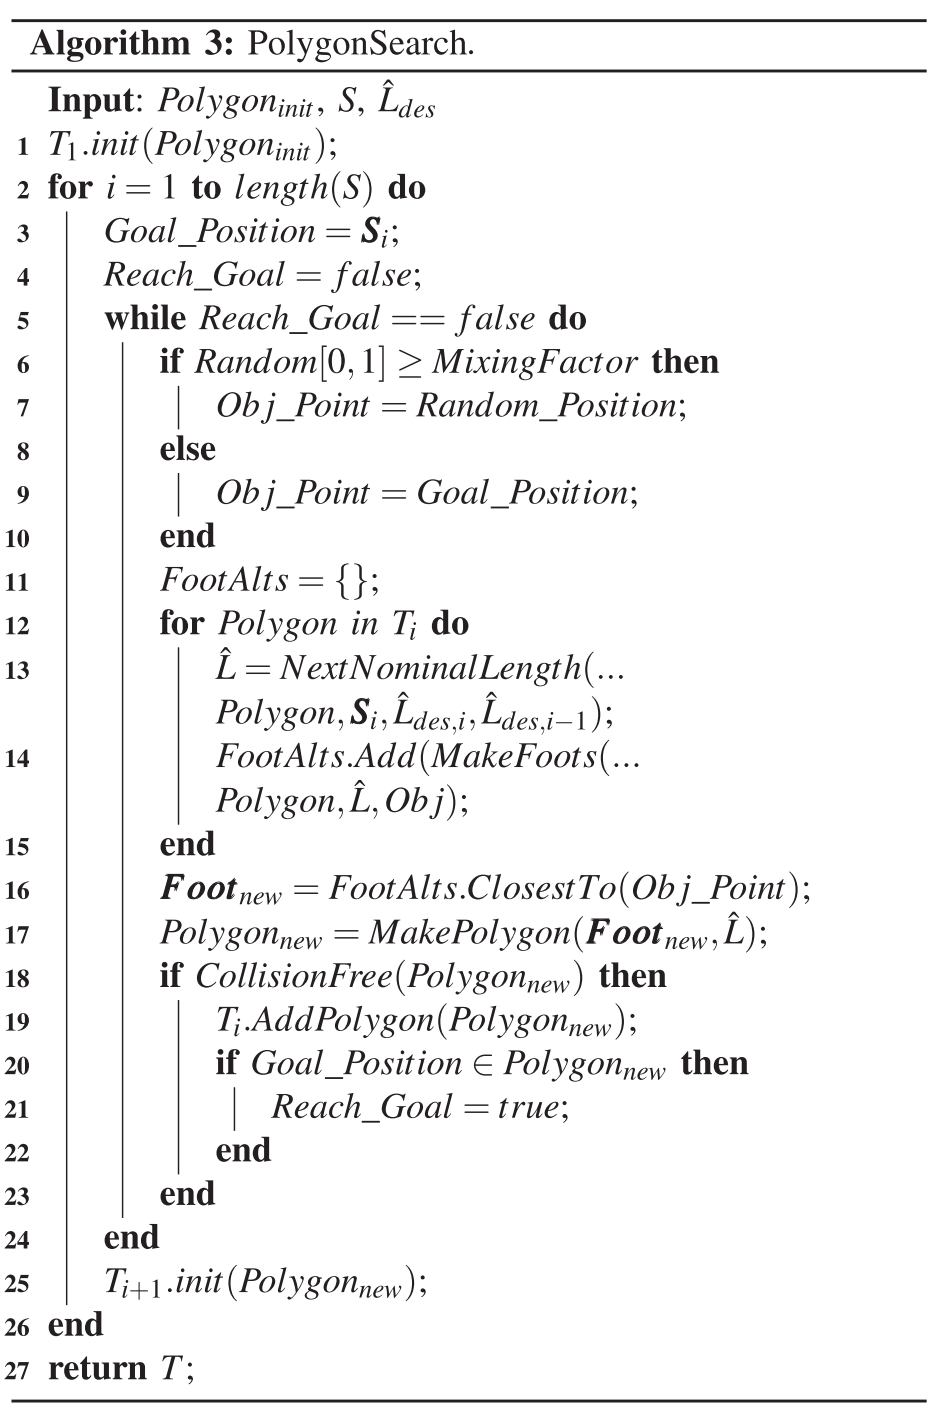
\includegraphics[height=72mm]{elements/[23]-PRT-V.png}
        \end{textblock*}

        \begin{textblock*}{88mm}(0mm,-20mm)
        The variable size aspects builds upon the previous planning, modifying the algorithm slightly with added higher level steps such called prior planning.
        \vspace{2mm}
        \begin{itemize}
            \item The stepover points are used as \alert{waypoints}.
            \item Each waypoint has a nominal robot size ($\hat{L}_{des}$) associated.
            \item Plan for paths between consecutive waypoints and interpolate the size of the polygons inbetween.
        \end{itemize}
        \end{textblock*}

        \begin{textblock*}{5cm}(133.4mm, 40mm) % {block width} (coords)
        {\tiny \cite{9477154}}
        \end{textblock*}

        \vspace{10mm}

\end{frame}

\begin{frame}[fragile]{\textbf{Simulation Results on PRT-V Algorithm}}
    
        \begin{textblock*}{5cm}(0mm,-22mm) % {block width} (coords)
        \href{https://youtu.be/MB3nqaDeuyU?si=1ECQ7Ujp21Hg77ce&t=5}{
        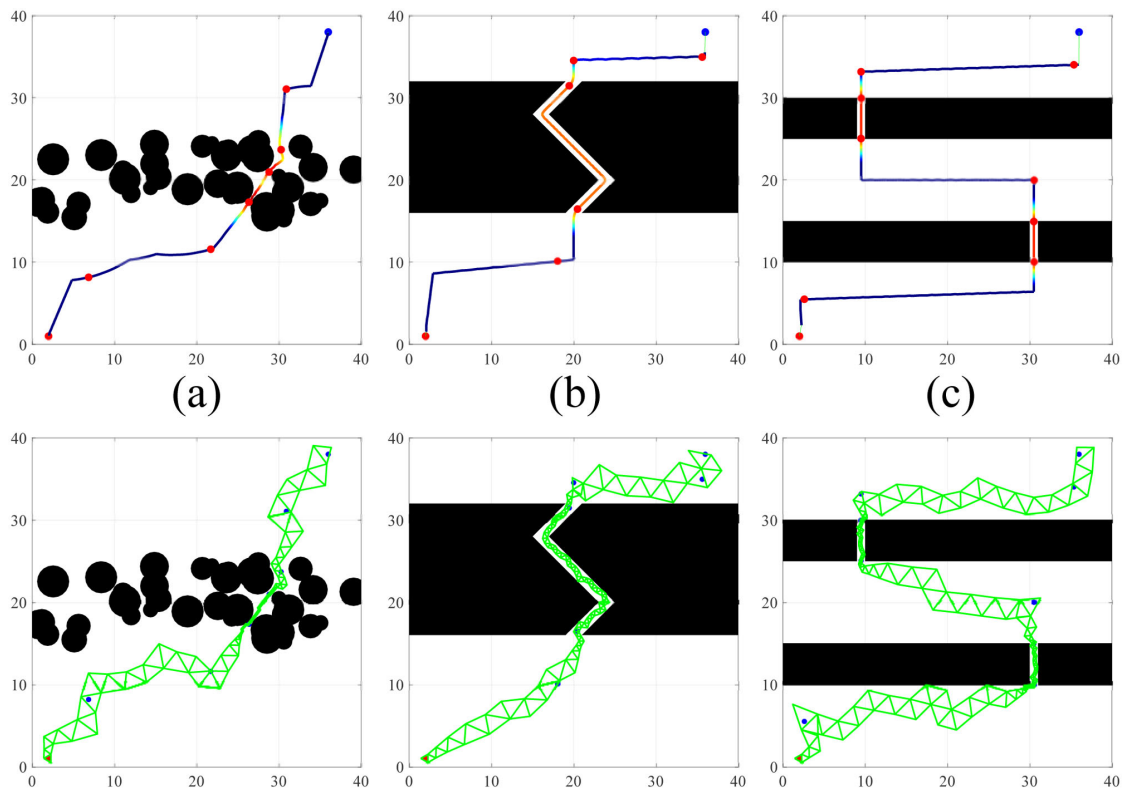
\includegraphics[height=58mm]{elements/[24]-PRT-V.png}}
        \end{textblock*}

        \begin{textblock*}{45mm}(85mm,-24mm)
        Discussions
        \vspace{2mm}
        \begin{itemize}
            \item Concerns on the minimum size of the robot passing through the path found from voronoi diagram
            \item Larger structure moves faster, however its easier to collide with the obstacles.
            \item Should the sampling density change when the search space become larger ? 
        \end{itemize}
        \end{textblock*}

        \begin{textblock*}{5cm}(83mm, 32mm) % {block width} (coords)
        {\tiny \cite{9477154}}
        \end{textblock*}

        % \vspace{10mm}

\end{frame}


\section{Contributions \& Future Work}

\begin{frame}[fragile]{\textbf{Implementation \& Future Works}}

    % \begin{textblock*}{5cm}(9mm,12.7mm) % {block width} (coords)
    % 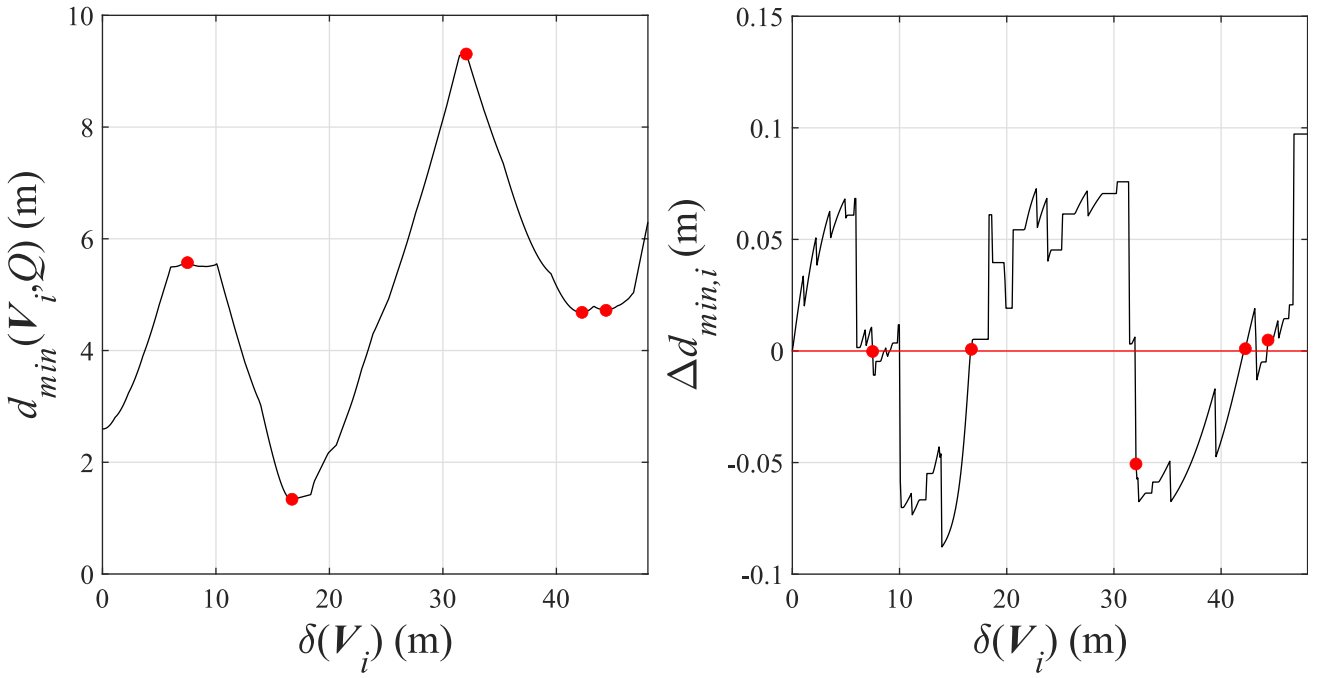
\includegraphics[height=30mm]{elements/[21]-PRT-V.png}
    % \end{textblock*}

    \begin{textblock*}{5cm}(46mm,8mm) % {block width} (coords)
    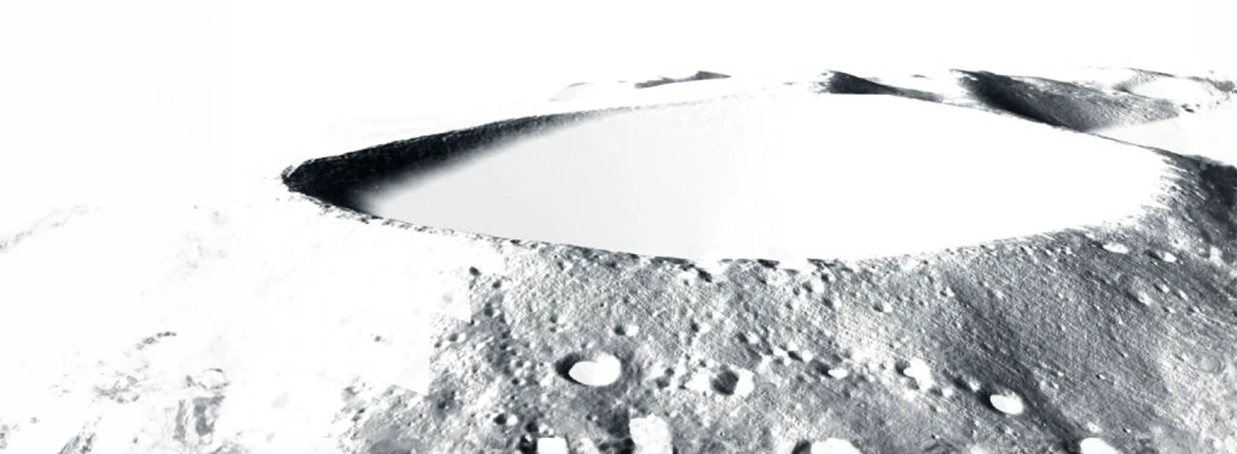
\includegraphics[height=34mm]{elements/[26]-Future.png}
    \end{textblock*}

    \begin{textblock*}{130mm}(0mm,-20mm)
    % One of the advantages of the physical topology is the \uline{size changing aspect}. The setting is still the same, but the question is when to change the size ?
    \vspace{2mm}
    \begin{itemize}
        \item The implementation will be conducted using MATLAB™, with dynamic simulation and visualizations performed in Rhino/Grasshopper®.
        \item Evaluate and document the generalizability of the pipeline for robots with various topologies.
        \item Modify locomotion and path planning 
        strategies to accommodate \\ 
        irregular non-planar terrains.
        \item Develop an approach for stair climbing \\
        and navigation in 2.5D environments.
    \end{itemize}
    \end{textblock*}

    \begin{textblock*}{5cm}(133mm, 38mm) % {block width} (coords)
    {\tiny \cite{9477154}}
    \end{textblock*}

    \vspace{10mm}

\end{frame}



% \begin{frame}[fragile]{Aspect ratio}

% 	The official ETH template only comes in 16:9.
	
% 	You can obtain 4:3 slides by passing the option \verb+aspectratio=43+
% 	\begin{verbatim}
% 		\documentclass[11pt,aspectratio=43]{beamer}	
% 	\end{verbatim}
		
% 	\bigskip
	
% 	In this case, you probably want to use the cover image \verb+\def\titlefigure{elements/title-page-image-43}+
% 	or any other image in 14:10 aspect ratio, for example \verb+\def\titlefigure{elements/title-page-image-alt-43}+
	
	
% \end{frame}

% \begin{frame}[fragile]{Font size}

% 	The font sizes match the official ETH template quite accurately when the default option \verb+11pt+ is used.
	
% 	\bigskip
	
% 	You can get slightly smaller or larger text by passing the options \verb+10pt+ or \verb+12pt+, respectively.
% 	\begin{verbatim}
% 		\documentclass[10pt,aspectratio=169]{beamer}
% 		\documentclass[11pt,aspectratio=169]{beamer}		% default
% 		\documentclass[12pt,aspectratio=169]{beamer}
% 	\end{verbatim}	
	
% 	\bigskip
% 	You can also fine-tune the font sizes by modifying the \verb+beamerfontthemeeth.sty+ file.

% \end{frame}

% \begin{frame}[fragile]{Colors}

% 	You need to pick these colors
% 	\begin{itemize}
% 		\item \texttt{accentcolor} (alert text, blocks)
% 		\item \texttt{titlefgcolor} (the box on the title page)
% 		\item \texttt{titlebgcolor} (the background on the title page, in case you don't use an image)
% 	\end{itemize}
% 	Use these commands at the beginning of the document
% 	\begin{verbatim}
% 		\colorlet{titlefgcolor}{ETHGreen}
% 		\colorlet{titlebgcolor}{ETHGreen}
% 		\colorlet{accentcolor}{ETHRed}
% 	\end{verbatim}

% 	\medskip

% 	\begin{tabular}{ll}
% 	\textcolor{ETHBlue}{\rule{4mm}{3mm}} ETH Blue &
% 	\textcolor{ETHGreen}{\rule{4mm}{3mm}} ETH Green \\
% 	\textcolor{ETHPurple}{\rule{4mm}{3mm}} ETH Purple &
% 	\textcolor{ETHGray}{\rule{4mm}{3mm}} ETH Gray \\
% 	\textcolor{ETHRed}{\rule{4mm}{3mm}} ETH Red &
% 	\textcolor{ETHPetrol}{\rule{4mm}{3mm}} ETH Petrol \\
% 	\textcolor{ETHBronze}{\rule{4mm}{3mm}} ETH Bronze
% 	\end{tabular}
	
% \end{frame}

% \begin{frame}

% 	\frametitle{Title}
% 	\framesubtitle{Subtitle}
	
% 	Text and some \alert{alert text}
	
% 	\[
% 	m_a^\top h(\cdot)
% 	\]
	
	
% 	\begin{itemize}
% 	\item list one
% 	\item list another one
% 		\begin{itemize}
% 		\item test 1
% 		\item test 2
% 		\end{itemize}
% 	\end{itemize}

% \end{frame}

% \section{Blocks and boxes}

% \begin{frame}{Title with no subtitle}

% 	\begin{block}{Large box}
% 	Notice that blocks are a bit larger than the text, that's intended.
% 	\end{block}
	
% 	Column environments also eat some margins. Use the option \texttt{[onlytextwidth]} if you want to align columns to the wide blocks.
	
% 	\begin{columns}[onlytextwidth]
% 	\begin{column}{0.45\textwidth}
% 		\begin{block}{Small box}
% 		With some more text
% 		\end{block}
% 	\end{column}
% 	\begin{column}{0.5\textwidth}
% 		Think outside the box!
% 	\end{column}
% 	\end{columns}

% \end{frame}

% \begin{frame}{And, of course, figures!}

% 	\begin{columns}
% 		\begin{column}{0.33\textwidth}
% 			\includegraphics[width=\columnwidth]{example-image-a}
% 		\end{column}
% 		\begin{column}{0.33\textwidth}
% 			\includegraphics[width=\columnwidth]{example-image-b}
% 		\end{column}
% 		\begin{column}{0.33\textwidth}
% 			\includegraphics[width=\columnwidth]{example-image-c}
% 		\end{column}
% 	\end{columns}

% \end{frame}

% \begin{frame}

% 	\frametitle{Tables}
% 	\framesubtitle{Don't use vanilla \LaTeX{}  tables please}
	
% 		\begin{center}
% 			\begin{tabular}{@{}llr@{}}
% 				\toprule\multicolumn{2}{c}{Item} \\
% 				\cmidrule(r){1-2}Animal & Description & Price (\$)\\
% 				\midrule
% 				Gnat  & per gram  & 13.65 \\
% 				& each      & 0.01 \\
% 				Gnu   & stuffed   & 92.50 \\
% 				Emu   & stuffed   & 33.33 \\
% 				Armadillo & frozen & 8.99 \\
% 				\bottomrule
% 			\end{tabular}
% 		\end{center}

% \end{frame}

% \section{URLs and links}

% \begin{frame}{Clickable links}

% 	Lorem ipsum dolor sit amet, consectetur adipiscing elit, sed do eiusmod tempor incididunt ut labore et dolore magna aliqua. 
% 	Ut enim ad minim veniam, quis nostrud exercitation...
	
% 	\medskip

% 	\url{http://control.ee.ethz.ch}
	
% 	\href{http://control.ee.ethz.ch}{Automatic Control Laboratory}
	
% 	\email{name@ethz.ch}

% \end{frame}

\begin{frame}[allowframebreaks]{Bibliography}
    \setbeamercolor{bibliography}{fg=black}
    \bibliographystyle{ieeetr}
    \bibliography{refs.bib}
\end{frame}

\begin{closingframe}
    \smallskip
    {\Large Thank you for listening}
    % \begin{textblock*}{5cm}(50mm,-5mm) % {block width} (coords)
    % 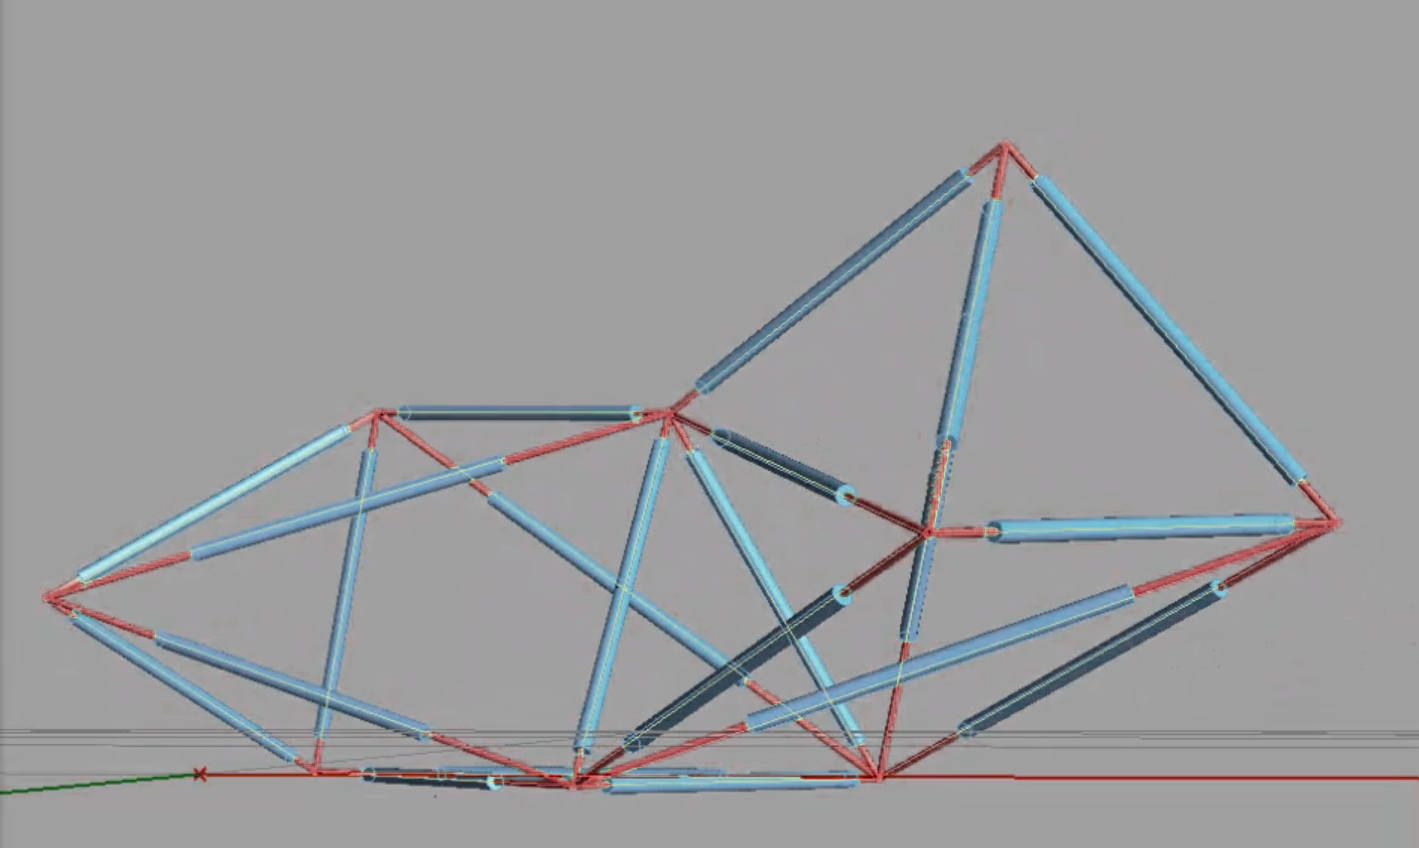
\includegraphics[height=50mm]{elements/[25]-Future.png}
    % \end{textblock*}
    \medskip
    \vspace{10mm}
\end{closingframe}


% \begin{closingframe}

% 	You can edit the content of the \texttt{closingframe} environment to design your own closing frame. Example:
	
% 	\vspace{15mm}

% 	\begin{columns}
% 		\begin{column}{0.55\textwidth}
% 			\raggedleft
% 			
\includegraphics[width=45mm]{elements/IFA_logo_ENG_colours_horizontal} 
% 		\end{column}
% 		\begin{column}{0.45\textwidth}
% 			\textbf{Author name}\\
% 			\email{name@ethz.ch}	
% 		\end{column}
% 	\end{columns}

% 	\vspace{20mm}
			
% \end{closingframe}


\end{document}